% !TEX program = xelatex

% Joint Programme with University of Information Technology, VNU-HCM
% Module: Individual Honours Project
%
% -----
%
% A Game-Based Approach to Motor Imagery Adaptation and BCI Calibration
% Author: Cao Đăng Khoa (dang.cao@mail.bcu.ac.uk)
% Student ID: 25195675
%
% Supervisor: Dr. Vi Chí Thành (vcthanh@hcmiu.edu.vn)
%------------------------------------%



%------ DOCUMENT CONFIGURATION ------%
\documentclass[a4paper, 11pt, openany]{report}
\usepackage{layout}
\usepackage{fonts}
\usepackage{headerfooter}
\usepackage{frontmatter}
\usepackage{contents}
\usepackage{atbegshi}
\usepackage[round, authoryear]{natbib}
\usepackage{graphicx}
\usepackage{booktabs}
\usepackage{array}
\usepackage{amsmath}
\usepackage{float}

% Hyperref for clickable links in TOC, LOF, LOT, and citations
\usepackage[
    colorlinks=true,
    linkcolor=black,
    citecolor=black,
    urlcolor=blue,
    bookmarks=true,
    bookmarksopen=true,
    pdfstartview=FitH
]{hyperref}



% Make \cite produce (Author, Year)
\let\cite\citep

\makeatletter
\let\ps@plain\ps@fancy
\makeatother


%------------------------------------%



%----------- FRONT MATTER -----------%
\begin{document}

% Title Page
\reportTitlePage
    {Final Report}
    {BCG: A Game-Based Approach to Motor Imagery Adaptation and BCI Calibration}
    {Cao Đăng Khoa}{25195675}
    {Bachelor of Science with Honours Computer Science}
    {Dr. Vi Chí Thành}{June 8, 2026}
    \thispagestyle{titlepage}

% Page numbering
\pagenumbering{roman}
\setcounter{page}{0}

% Abstract
\reportAbstract{
    Brain-Computer Interfaces (BCIs) enable direct communication between the human brain and external devices through neural signals. While Motor Imagery-based BCIs have demonstrated promising applications in rehabilitation and assistive technology, their widespread adoption remains limited by a critical bottleneck: the calibration process. Traditional calibration protocols require 15-30 minutes of repetitive, supervised training per session, inducing cognitive fatigue and limiting real-world scalability. This project addresses this limitation by investigating a game-based approach to BCI calibration. A dual-mode software framework is developed to compare two data collection protocols: the Standard Graz Protocol (traditional) and a Gamified Calibration Protocol (proposed). The system integrates real-time EEG signal processing with an engaging game interface, allowing calibration data to be collected implicitly during gameplay within the software architecture. A between-subjects user study with healthy participants evaluates the comparative effectiveness by measuring subjective workload (NASA-TLX) and boredom levels. Preliminary findings suggest that gamification may reduce perceived calibration workload and fatigue while establishing a functional software architecture for automated data labeling, offering a practical pathway toward more accessible and user-friendly brain-computer interaction systems.
}

% Acknowledgements
\reportAcknowledgements{
    Before starting the main content of this dissertation, I want to take a moment to express my deep appreciation to all those who supported me throughout this project.
    
    First and foremost, I would like to express my deepest gratitude to my supervisor, Dr. Vi Chi Thanh, for giving me the opportunity to work with EEG-Based Brain-Computer Interface, a field that is still very new and hard to access in Vietnam. He was always open to helping me and provided the best conditions for me to complete this project. Additionally, I would like to thank Ms. Trang for giving me valuable advice, writing guidance, and practical experience with the data collection process.
    
    I am also very grateful to Brain-Life and Emotiv for their crucial support with the research equipment. Brain-Life gave me the opportunity to test various EEG devices and supported me by lending the main EEG device for this project. Emotiv sponsored the software license that allowed me to access and collect raw EEG data.
    
    Next, I want to send my deepest love and thankfulness to my Mom and my family. My Mom has always been my strongest supporter. Her daily hard work and dedication gave me the peace of mind to focus on my studies and chase my dream. I also want to mention my main source of mental strength - my close friends, whom I consider my brothers. Thank you all for always listening, understanding, and having my back.
    
    Finally, I would like to thank myself for staying persistent throughout this journey and for overcoming the challenges I faced along the way.
    
}

% Abbreviations
\reportAbbreviations{
\begin{tabular}{@{}ll@{}}
\textbf{BCI} & Brain-Computer Interface \\
\textbf{EEG} & Electroencephalography \\
\textbf{MI} & Motor Imagery \\
\textbf{ERD} & Event-Related Desynchronisation \\
\textbf{ERS} & Event-Related Synchronisation \\
\textbf{CSP} & Common Spatial Patterns \\
\textbf{LDA} & Linear Discriminant Analysis \\
\textbf{SVM} & Support Vector Machine \\
\textbf{HCI} & Human-Computer Interaction \\
\textbf{NASA-TLX} & NASA Task Load Index \\
\textbf{LOTO} & Leave-One-Trial-Out \\
\end{tabular}
}

% Table of Contents
\reportTableOfContents

% List of Figures
\reportListOfFigures

% List of Tables
\reportListOfTables
%------------------------------------%


\cleardoublepage
\pagenumbering{arabic}

% Main content formatting: 1.5 line spacing, double-space between paragraphs
\setstretch{1.5} 
\setlength{\parskip}{10pt plus 2pt minus 1pt} 

% \setstretch{1.2} 
% \setlength{\parskip}{8pt plus 2pt minus 1pt} 

%------------ CHAPTER 1 -------------%
%----- Introduction and Context -----%
\vspace*{-1.15cm}
\chapter{Introduction}

    % 1.1 Background 
    \section{Background}

    The way humans interact with computers has undergone a significant evolution over time. From keyboards and mice to touch screens and voice assistants, each innovation has expanded how people engage with digital systems. Brain-Computer Interfaces (BCIs) represent the next frontier: systems that enable people to control devices directly with their thoughts. By translating neural signals into digital commands, BCIs not only enhance experiences for typical users but also provide communication and control pathways for people with severe motor disabilities \cite{wolpaw2002brain, kubler2001brain}.  
    
    Among BCI paradigms, electroencephalography-based motor imagery (EEG-MI) is one of the most widely studied \cite{lotte2018review}. When a person imagines a movement, such as moving their left or right hand, without physically performing it, the brain still produces neural signals remarkably similar to those during actual execution \cite{jeannerod1995mental, neuper2001event}. This principle underpins a broad range of real-world applications, including motor rehabilitation, assistive device control, and interactive gaming. These promising applications, however, still depend heavily on how accurately MI signals can be detected, with the calibration process playing a crucial role.


    % 1.2 Current State and Limitations
    \section{Current state and limitations}

    In controlled laboratory environments, EEG-MI systems demonstrate a high level of performance, often reaching accuracies above 
    70\% \cite{wolpaw2002brain, kubler2001brain}. Despite this strong laboratory performance, real-world 
    adoption faces a critical barrier: the dependency on long, repetitive per-session calibration. Because MI signals are non-stationary 
    and vary significantly between individuals and across sessions \cite{sugiyama2007covariate, lotte2018review}, a classifier trained in one session may fail in 
    the next.

    The standard approach, the Graz calibration protocol, requires 15 to 30 minutes of supervised, cue-driven trials per session \cite{giles2022transfer, kueper2024avoidance}, 
    collecting 40 to 80 labeled trials per movement class, totaling around 120-240 trials. Users watch directional 
    prompts on a screen and imagine the corresponding movement on command. This process induces cognitive fatigue that progressively 
    degrades the very signal quality it is trying to capture. It also requires specialist supervision and depends on 
    laboratory infrastructure, keeping this technology largely confined to clinical settings rather than achieving widespread adoption.


    % 1.3 Problem Statement
    \section{Problem statement}

    Motor Imagery (MI) has not yet achieved widespread application primarily due to the strict limitations of the standard calibration phase. 
    This initial setup is heavily bottlenecked by brain signal variations across different sessions and individuals, 
    the necessity for constant human supervision, and a strong reliance on specific laboratory infrastructure. Consequently, users must endure
    a fatiguing and repetitive process precisely when the system requires the highest-quality data.

    While gamification effectively improves user engagement and signal quality, it is rarely utilized during this critical calibration phase. 
    To resolve this, this project introduces BCG: a game-based calibration system. BCG applies engagement mechanics directly to the data 
    collection process, designed to naturally gather and reliably label MI trials without relying on monotonous, explicit prompts.


%------------------------------------%

%------------ CHAPTER 2 -------------%
%--- Review of Existing Knowledge ---%


\chapter{Review of Existing Knowledge}

    % 2.1 The Neuroscience of Motor Imagery
    \section{The neuroscience of motor imagery and EEG processing}
    To interpret human intention, we must examine the concept of functional 
    equivalence. Modern research has shown that planning a movement and 
    physically performing it are not distinct processes \cite{jeannerod1995mental}. 
    When a person performs Motor Imagery, mentally imagining a movement while 
    remaining physically still, their brain activates many of the same neural 
    networks used during actual execution.

    When a user imagines moving a limb, such as their right hand, the primary 
    motor cortex generates specific, rhythmic electrical patterns. These patterns 
    occur in the sensorimotor cortex and are governed by the contralateral 
    principle: imagining a right-hand movement primarily activates the left 
    hemisphere, while left-hand imagery activates the right \cite{jeannerod1995mental, wolpaw2002brain}.

    \begin{figure}[h]
        \centering
        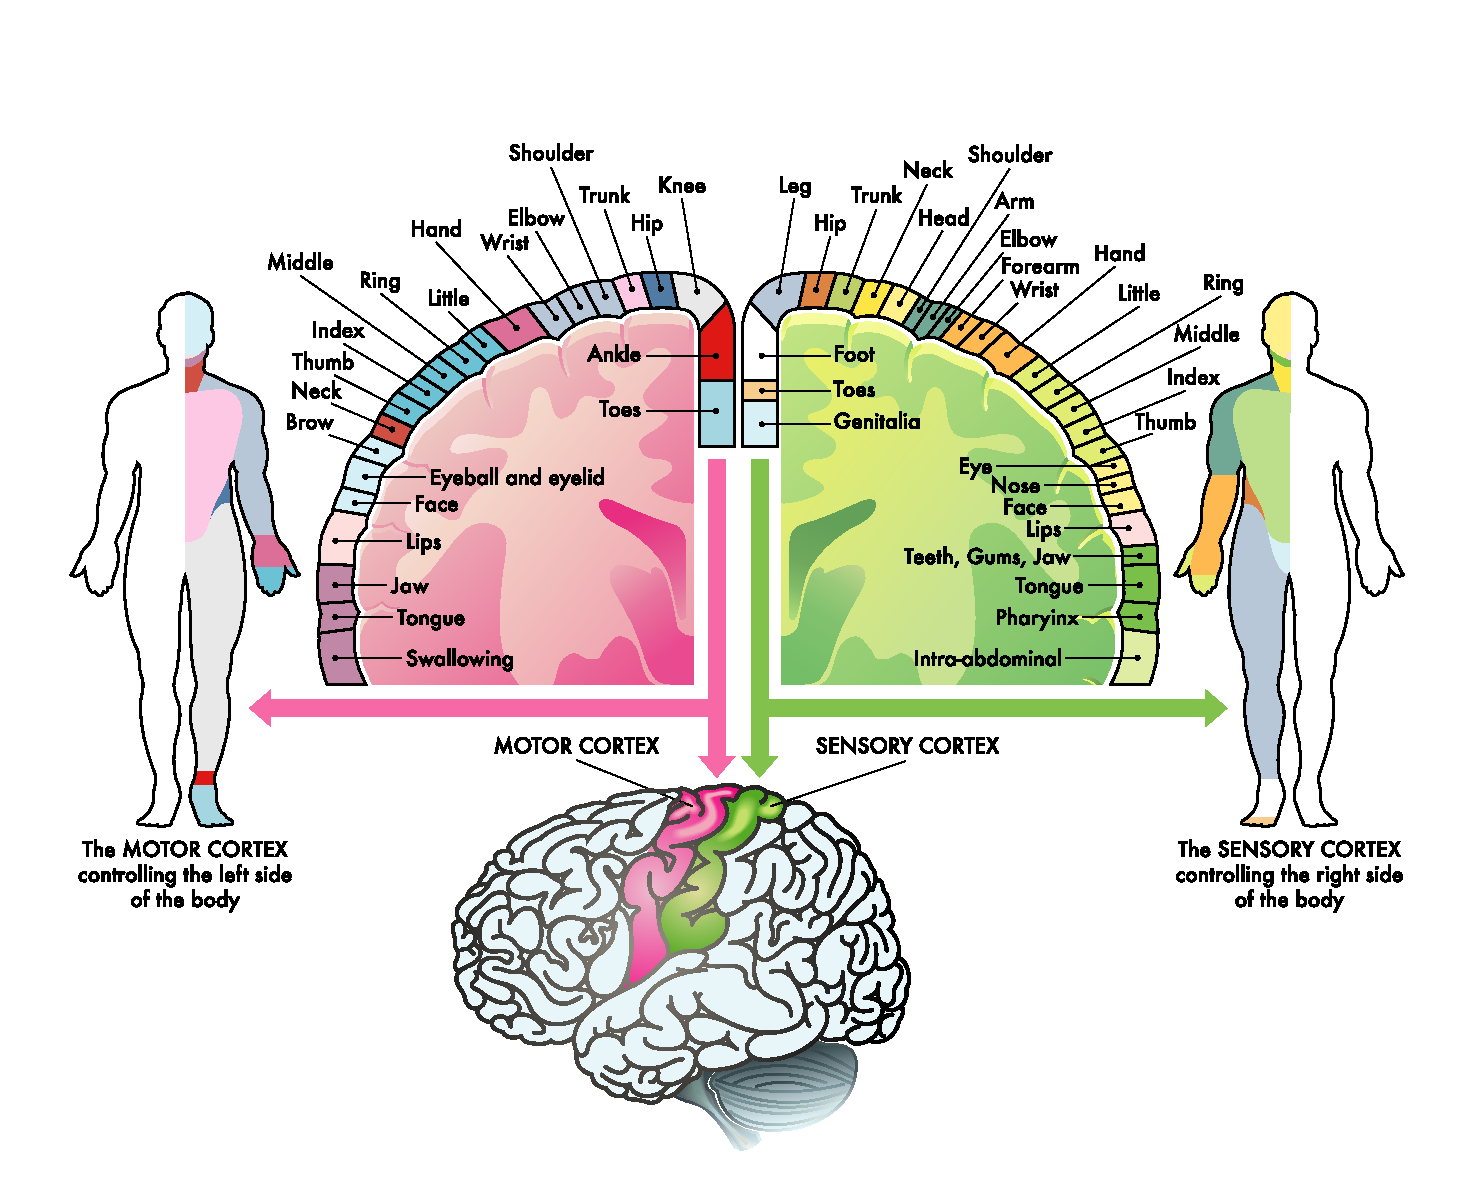
\includegraphics[width=1\textwidth]{Images/neuroscience-of-motor-imagery.pdf}
        \caption{Motor Cortex Organization and Contralateral Hemispheric Control}
        \label{fig:neuroscience-of-motor-imagery}
        \end{figure}
        
        
    These activations are measurable through changes in brain rhythms. In a 
    resting state, neurons fire in synchrony, creating strong idle rhythms known 
    as Mu (8-13 Hz) and Beta (13-30 Hz). When the user begins imagining movement, 
    this synchrony is disrupted, causing a power drop known as Event-Related 
    Desynchronisation (ERD). Conversely, when the brain relaxes, the neurons 
    synchronise again, leading to Event-Related Synchronisation (ERS) \cite{pfurtscheller1999event, neuper2001event}.

    These ERD/ERS patterns are the core signatures BCI systems are trained to 
    recognise. While they are highly reproducible and occur even in individuals 
    with severe motor disabilities, their specific structure varies significantly 
    between individuals. The frequency and spatial distribution 
    of these signals are unique to each person, necessitating a system that can 
    adapt to the user.

    Capturing these tiny biological signals without surgery is an engineering challenge 
    because the signals are often hidden by muscle movements and background electrical noise. 
    To address this, the data must go through a processing pipeline. First, digital bandpass 
    filters keep only the 8 to 30 Hz frequencies, removing unwanted noise. Once the data 
    is cleaned, the system extracts the necessary patterns, preparing the signals for machine 
    learning algorithms to classify the user's intention.
    



    \section{The Graz data collection protocol}
    The Graz protocol is currently the most common method for collecting labeled BCI data in 
    laboratories \cite{wolpaw2002brain, lotte2018review}. A typical session is strictly timed and very repetitive. First, a cross 
    appears on a screen to tell the user to get ready. Then, an arrow points left or right, 
    instructing the user to imagine moving that hand for 4 to 6 seconds. While this method 
    creates very clean data in a lab, it is the main reason why BCIs struggle to be used in 
    the real world.

    Extended exposure to repetitive directional prompts induces user fatigue and reduces sustained attention. 
    When users experience cognitive disengagement, their brain signals become attenuated and inconsistent. 
    This creates a negative feedback loop: degraded signal quality produces suboptimal training data, 
    which in turn leads to reduced classifier performance and increased user frustration. Furthermore, brain 
    signals exhibit high intra-subject variability across sessions depending on arousal and attentional state \cite{giles2022transfer}. 
    Because of this, users must complete this demanding 15 to 30 minute calibration procedure at the beginning 
    of every single session, repeating the task 120 to 240 times just to initialize the system.



    \section{Gamification, covert cues, and the labeling problem}
    To solve this fatiguing process, researchers have used gamification, adding game elements to BCI tasks 
    to keep users motivated. Studies show that when users are engaged in a game and enter a psychological 
    "flow state", they pay better attention. This creates much clearer brain signals compared to following 
    tedious directional prompts \cite{skola2019progressive, atilla2024gamification}. However, most current BCI software only uses gamification for the training 
    phase. The initial calibration step remains unchanged because it still relies on forcing the user to 
    follow direct commands.

    To successfully bring gamification into this calibration phase, a better solution is to stop giving 
    explicit instructions and use implicit, task-driven events instead. Research has established that 
    natural game interactions can successfully trigger specific brain signals \cite{vi2012detecting}. This "covert cue" idea 
    suggests we can hide the calibration step inside a game. Instead of telling the user to imagine 
    moving a hand, the game simply creates a situation where the player naturally imagines that movement 
    to win.
    
    However, using a game for calibration creates a major challenge: the labeling problem. In machine 
    learning, every piece of brain data must be perfectly matched with a label, such as "Left Hand". 
    If a game allows players to move freely or choose from many options, the system cannot know exactly 
    what the user was intending to do at a specific second. This makes it impossible to automatically 
    label the data without a human checking it later.

    \section{Classification algorithms in motor imagery}
    The primary goal of collecting accurately labeled calibration data is to train the classification 
    algorithm. Traditionally, methods like Linear Discriminant Analysis (LDA) and Support Vector Machines 
    (SVM) have been widely used. These models remain highly valuable because they are computationally 
    efficient and perform well with limited datasets \cite{blankertz2008optimizing, lotte2018review}. However, because they often rely on fixed patterns 
    extracted during a single session, they can struggle to maintain accuracy when the user's brain signals 
    naturally change over time.

    Alternatively, deep learning approaches are increasingly explored to address these limitations \cite{lawhern2018eegnet}. Neural 
    networks can automatically extract spatial and temporal patterns directly from the raw data, and they 
    offer the potential to fine-tune a pre-trained model for a new user. Nevertheless, deep learning architectures 
    introduce their own challenges, such as higher computational demands and a strict dependency on large 
    volumes of data. Regardless of the chosen algorithm, whether a system employs traditional methods or 
    neural networks, its success heavily relies on the ability to consistently collect high-quality, accurately 
    labeled data during the initial setup phase.

    \section{Critical analysis and gap identification}
    Despite advances in BCI classification algorithms, practical application 
    remains 
    constrained 
    by the calibration 
    bottleneck. While gamification is known to improve user engagement and signal quality, it is rarely applied 
    to the calibration phase itself. This limitation is largely due to the technical difficulty of maintaining 
    controlled data collection. As a result, the literature currently lacks frameworks that replace the 
    standard, repetitive calibration protocol with an engaging alternative. Specifically, there remains a 
    need for practical methods that can seamlessly collect and automatically label data without sacrificing 
    reliability.

    \section{Project justification}
    This project directly addresses the identified gap by proposing a gamified calibration workflow that replaces explicit, fatiguing prompts with covert cues. By developing a system that naturally guides the user through game mechanics, this approach ensures that high-quality MI data can be seamlessly collected and properly labeled in the background.

    Beyond laboratory settings, this framework holds practical relevance for the development of user-centric BCI applications. Currently, deploying BCI software outside of clinical environments is heavily constrained by the strict requirements and poor usability of standard setup protocols. By demonstrating that calibration can be conducted efficiently while reducing user cognitive fatigue, this project offers a methodological step toward overcoming the calibration bottleneck, paving the way for more accessible and engaging BCI applications.

% ------------------------------------%

%------------- CHAPTER 3 -------------%–
%-Project Aims, Objectives, and Scope-%
\chapter{Project Aims, Objectives, and Scope}   

    % 3.1 Project Aim
    \section{Project aim}    
    The aim of this project is to develop and technically evaluate BCG, a gamified calibration 
    framework for Motor Imagery Brain-Computer Interfaces, focusing on its ability to utilize 
    covert cues to seamlessly collect and automatically label high-quality EEG data without 
    relying on explicit prompts.

    % 3.2 Project Objectives    
    \section{Project objectives}    
    To achieve this aim, the project focuses on the following objectives:
    
    \begin{enumerate}
        \item \textbf{Framework development:} To design and implement a dual-mode BCI software 
        framework that supports two distinct data collection protocols: a baseline mode 
        replicating the traditional Graz protocol (Condition A) and a proposed gamified 
        mode using covert cues (Condition B).
        
        \item \textbf{User experience evaluation:} To conduct a between-subjects pilot study 
        measuring subjective workload (NASA-TLX) and boredom to evaluate fatigue mitigation.
        
        \item \textbf{Baseline classifier investigation:} To identify and evaluate a hardware-compatible 
        machine learning model using public datasets, establishing a baseline classifier optimized for 
        14-channel motor imagery 
        recognition to be considered for future calibration performance testing.

        \item \textbf{Adaptive pipeline integration:} To implement an automated data ingestion and fine-tuning mechanism, 
        establishing a continuous pipeline architecture capable of processing user calibration data for model personalization. 
        Note that full closed-loop real-time inference remains constrained by thread synchronization challenges identified 
        during implementation.
    \end{enumerate}
        
    % 3.3 Project Scope    
    \section{Project scope}    
    The project boundaries are defined to ensure the feasibility of the 
    comparative study within the academic timeline.
    
    \textbf{In-Scope:}
    \begin{itemize}
        \item The design and implementation of the dual-mode BCI software framework, encompassing both the standard Graz protocol interface and the gamified environment utilizing covert cues.

        \item The design of a 2D game environment specifically for motor imagery tasks, including the backend system for real-time data ingestion and automated labeling.

        \item Integration with commercially available EEG headsets to capture the raw brain data.

        \item The evaluation of the implicitly collected data's viability to verify technical performance.
    \end{itemize}
    
    \textbf{Out-of-Scope:}
    \begin{itemize}
        \item Hardware engineering or custom headset design: The project uses existing commercial equipment only.

        \item Novel machine learning algorithms: The project evaluates established methods rather than creating new ones.

        \item Training classifiers on self-collected data: The baseline model is trained on public datasets.

        \item Clinical trials or studies with patients: Evaluation is strictly limited to healthy participants.

        \item Comparing classification accuracy between Graz and game conditions: The focus is on user experience (NASA-TLX) and technical pipeline validation.

        \item Long-term studies or formal statistical hypothesis testing: The pilot study aims for preliminary feasibility only.
    \end{itemize}


\chapter{Project Design and Experimental Methodology}
    This chapter outlines the conceptual design of the comparative calibration platform. It focuses on the human-computer interaction (HCI) approach, the game mechanics used to solve the EEG data labeling challenge, and the overall setup for the user study.


    % 4.1 Conceptual Framework: MI-as-Data-Collection
    \section{Conceptual framework: MI-as-Data-Collection}
    
    Before designing the interaction, it is necessary to distinguish between two different types of motor imagery-based games. The BCG platform belongs to the latter category, where gameplay serves the calibration process to learn the user's brain patterns before real-time prediction starts.

    \begin{itemize}
        \item \textbf{MI-as-Control:} In this approach, a fully trained model controls the game in real time. The player uses their brain signals as an input device, and the game is built around the model's capabilities.

        \item \textbf{MI-as-Data-Collection:} In this approach, playing the game functions as a structured protocol to collect labeled EEG data to train or update a model. The main goal is to gather accurate data while the user performs an interactive task, rather than providing a perfect gaming experience.
    \end{itemize}


    % 4.2 Game Mechanic Design and the Labeling Problem
    \section{Game mechanics design and the labeling problem}
    
    A major challenge in creating a data-collection game is ensuring the data labels are accurate. To train an AI model properly, the system must know which motor imagery task the player is focusing on at any exact moment. If a game gives the player too many options, such as a three-lane track where a player can dodge left, right, or stay in the middle, the system cannot accurately guess the player's intention before a personal model is trained. This uncertainty means the system might label the data incorrectly, making it unusable for the calibration process.

    To resolve this issue, BCG strictly limits the game interface to exactly two lanes. During each trial, a note falls down either the left or the right lane. Because the game forces a simple binary reaction, the player's response is highly predictable. The correct ground-truth label is decided entirely by which lane the note appears in. This guarantees accurate data labels without requiring an expert to manually verify them later. It is important to acknowledge, however, that this automated labeling approach assumes participants comply with the motor imagery instruction during gameplay. The system cannot directly verify whether users are genuinely performing motor imagery or relying on alternative cognitive strategies such as visual attention or reflexive responses. This assumption represents a methodological limitation inherent to covert-cue designs.


    % 4.3 Hidden cues and mental workload reduction
    \section{Hidden cues and mental workload reduction}
    
    By restricting the game to two lanes, the design naturally acts as a system of hidden, or covert, cues. Instead of showing direct text instructions on the screen like ``imagine your left hand''—which is common in the standard Graz protocol—BCG puts the player in a situation where playing the game naturally creates the exact motor imagery signal the system needs to record.

    Consequently, the user is guided to perform the mental tasks without feeling like they are participating in a strict laboratory test. This design shifts their mental focus away from following rigid commands and toward simply matching a rhythm. This approach aims to produce more natural EEG signals that are less affected by boredom or experimental stress.


    % 4.4 Experimental Setup for User Study
    \section{Experimental setup for user study}
    
    To evaluate how well this design works, a user study is set up to compare the explicit Graz protocol with the implicit BCG game. The experiment follows a between-subjects design, where participants are randomly assigned to either the Graz group or the BCG group. This separation prevents learning effects and reduces the extra fatigue that would occur if one person had to complete both tests sequentially.

    To keep the comparison fair, both testing conditions are structured to collect exactly 78 EEG trials per person and last approximately 10 minutes. This ensures any difference in user experience comes directly from the interface design, rather than the length of the task. Right after the session, participants fill out the NASA-TLX survey to measure their cognitive workload, breaking down their fatigue into specific factors like mental demand and physical effort. They also report their boredom levels to show if the hidden game mechanics effectively reduce mental strain compared to the standard method.

\chapter{Artefact Design and Implementation}

    % 5.1 System Architecture and Project Structure
    \section{System architecture and project structure}

    % 5.1.1 System Components and Execution Flow
    \subsection{System components and execution flow}

    The platform uses a unified desktop launcher built with PyQt6. Instead of routing everything through a single background server, the launcher opens one of three desktop applications based on the user's choice: Graz Data Collect, Live MI Monitor, or Game Server Control Panel. As shown in the system architecture flowchart (Figure 5.1), these applications share a core logic library called \texttt{bcg\_core}, but they run differently to improve performance.

    For Graz data collection and Live MI monitoring, the applications run entirely on the local desktop, communicating directly with the core runtime using PyQt signals. However, their tasks differ. The Graz application only connects to the data streaming worker to record and save labeled trials. The Live MI monitor also connects the stream to the classification module for real-time predictions. This direct connection avoids network delays, keeping data collection and processing within a single app process.

    On the other hand, the game mode uses a client-server setup. The Game Server Control Panel starts the Python backend server on a separate background thread. Then, the browser game, built with HTML5 Canvas and JavaScript, connects to this backend via a local WebSocket. In this setup, the data streaming worker sends signals directly to the WebSocket server. The browser handles the interface and tracks trial events, sending exact timing and labels based on the game. Meanwhile, the Python backend handles data saving and model calibration.

    \begin{figure}[H]
    \centering
    \setlength{\fboxsep}{10pt}
    \setlength{\fboxrule}{0.1pt}
    \fbox{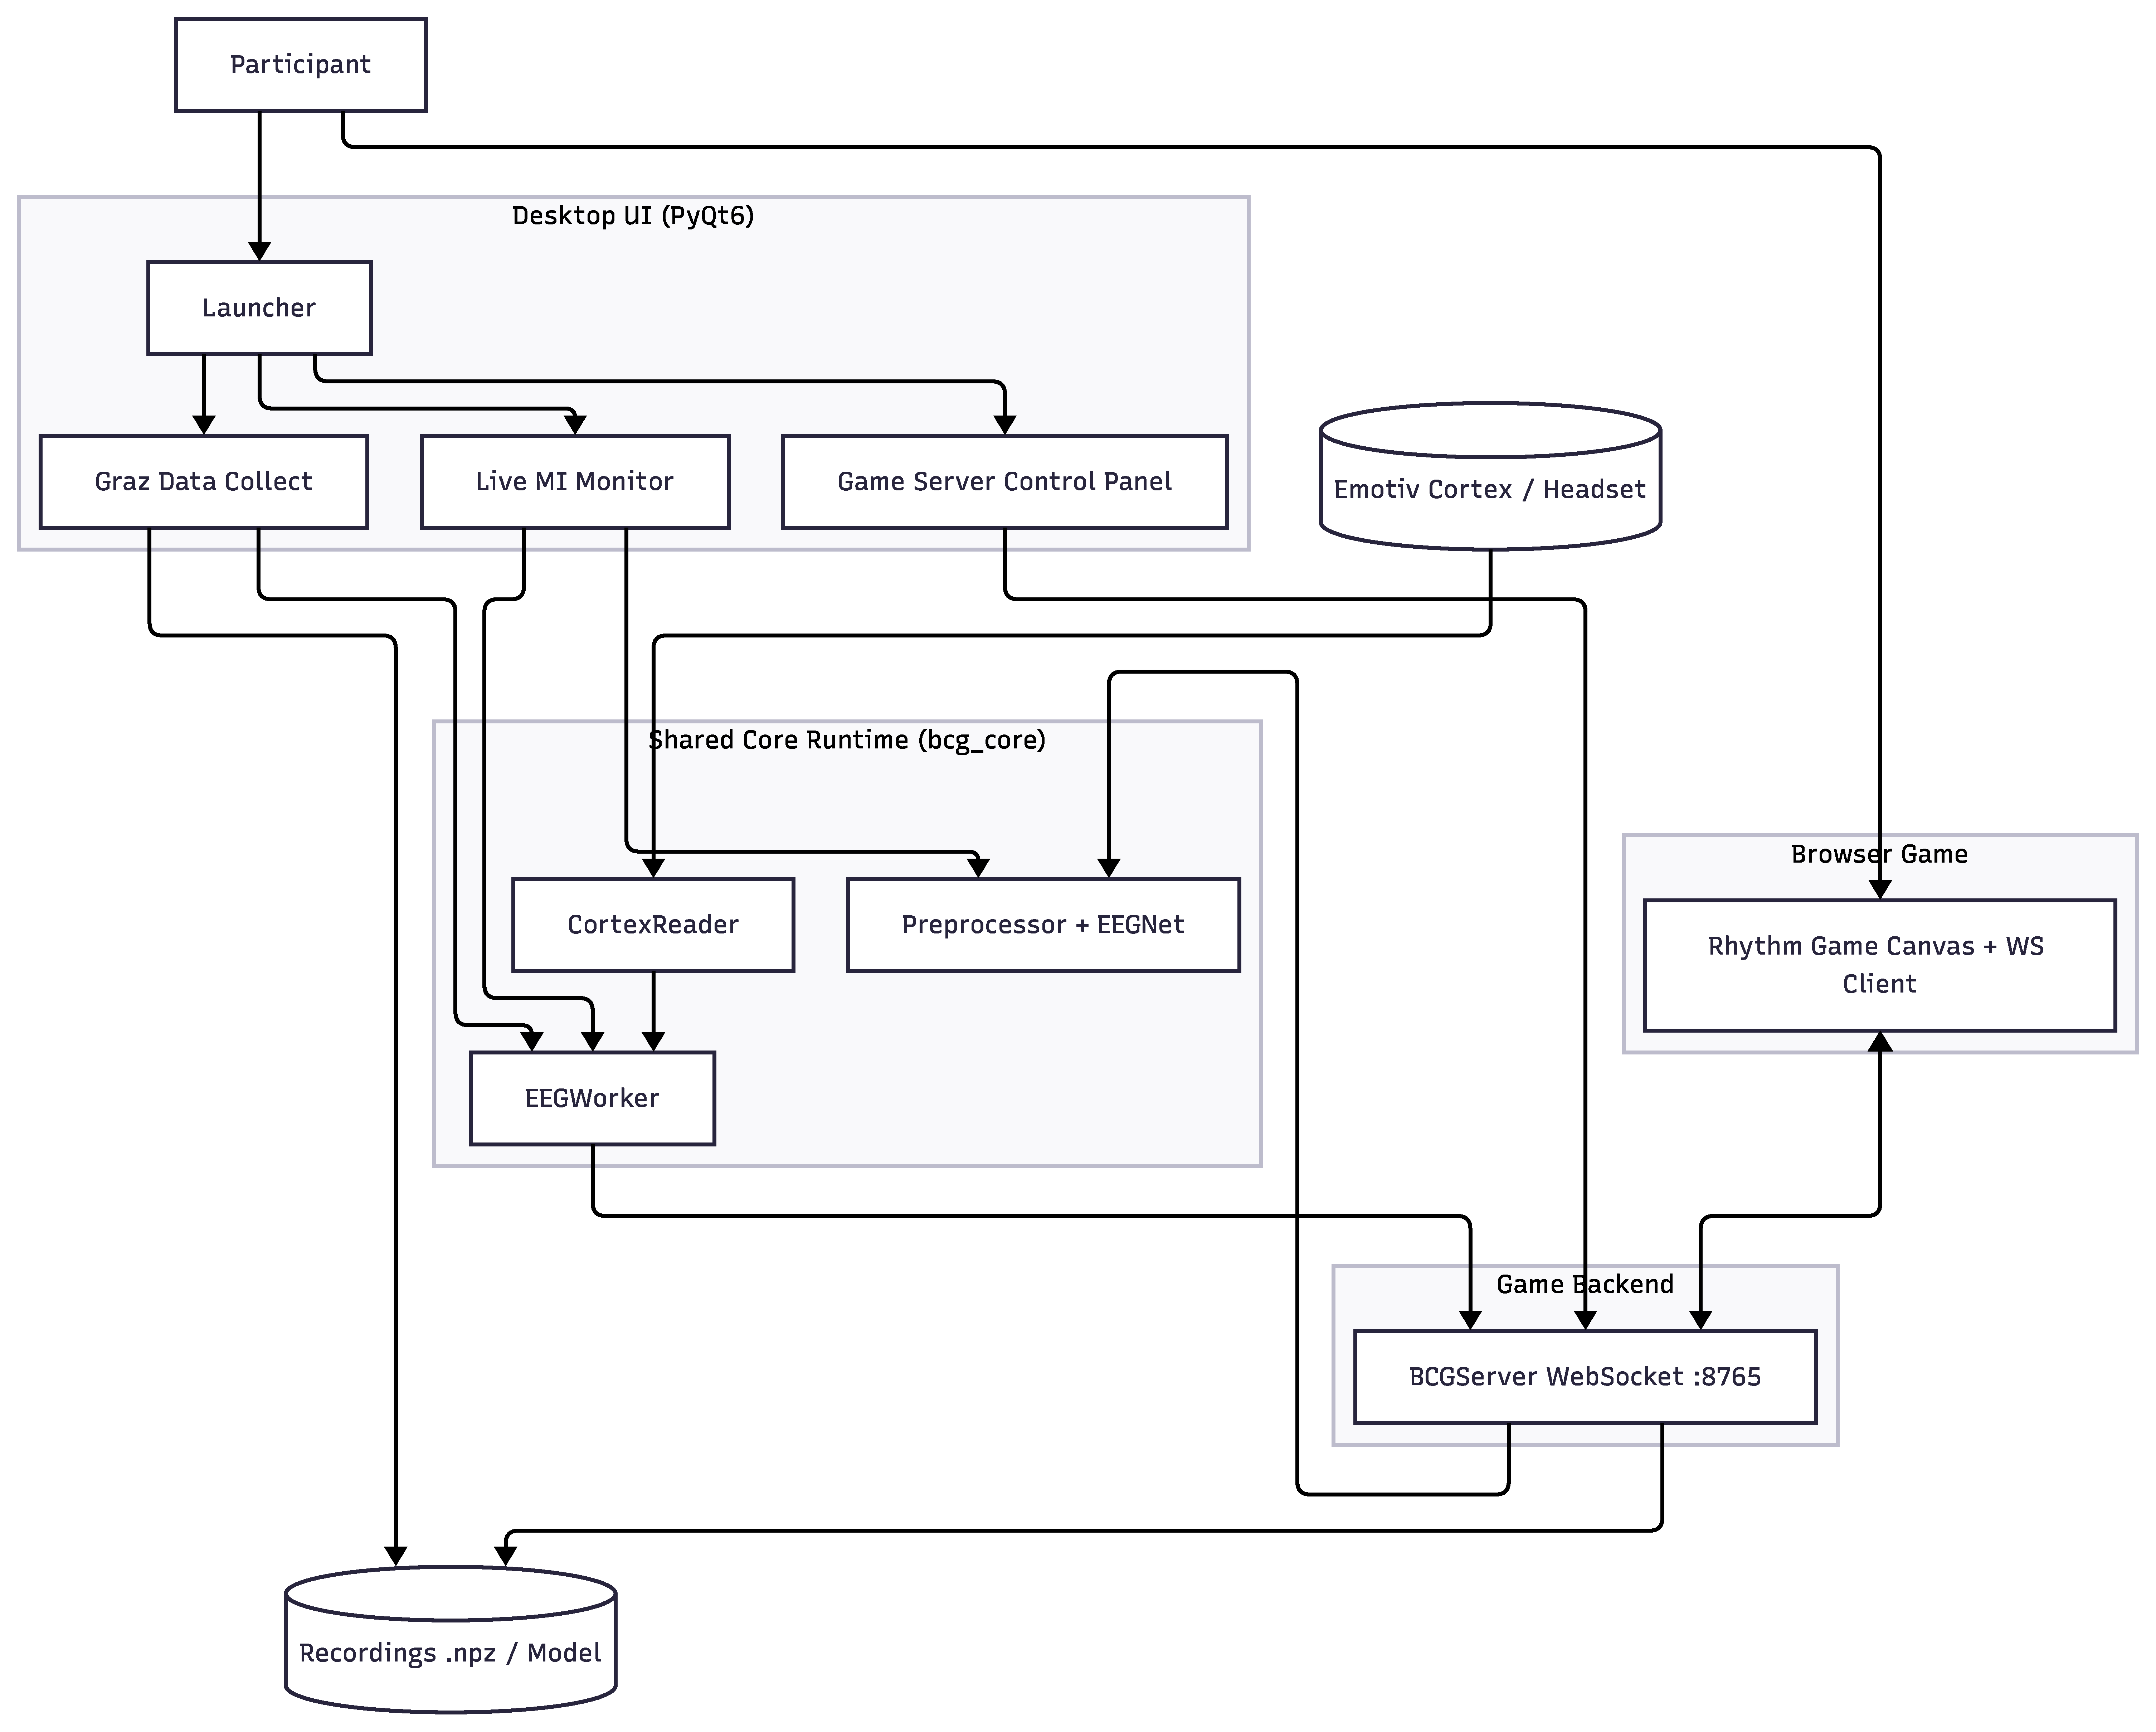
\includegraphics[width=0.98\textwidth]{Images/system-architecture-overview.pdf}}
    \caption{System Architecture Flowchart}
    \label{fig:system-architecture-overview}
    \end{figure}

    \begin{figure}[H]
    \centering
    \setlength{\fboxsep}{10pt}
    \setlength{\fboxrule}{0.1pt}
    \fbox{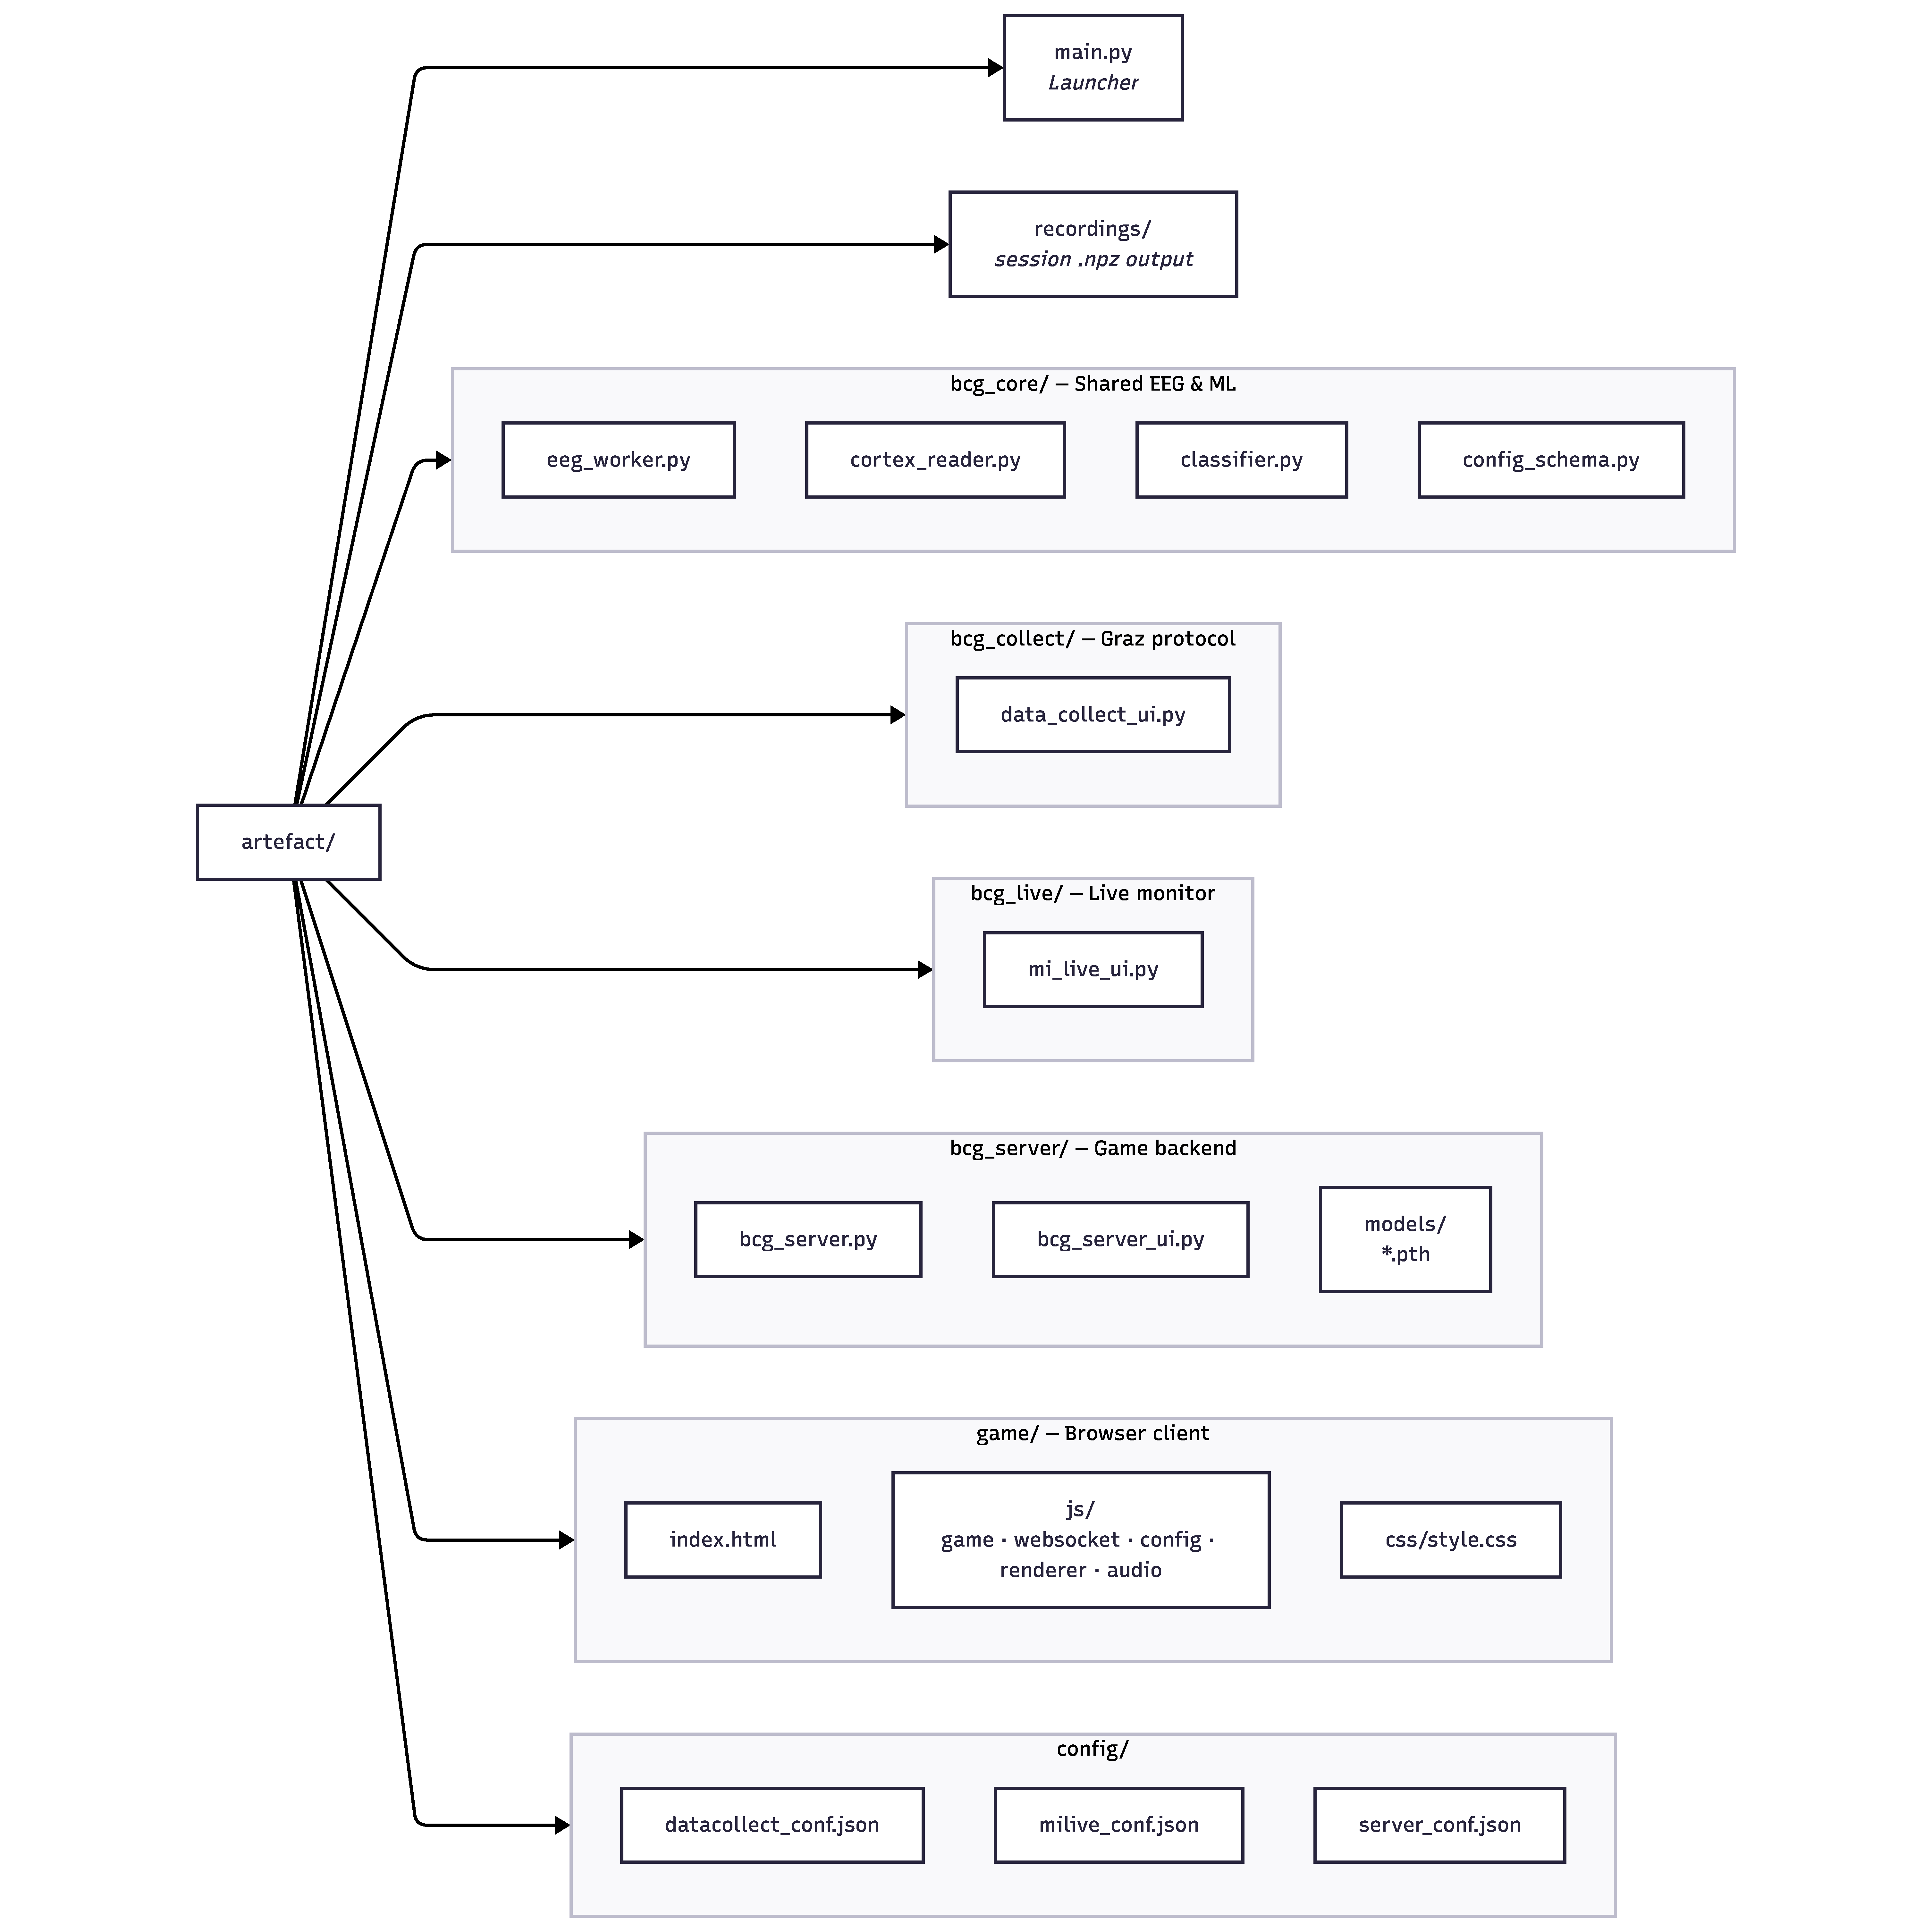
\includegraphics[width=0.98\textwidth]{Images/artefact-tree-diagram.pdf}}
    \caption{Directory Tree Diagram of the Project Repository}
    \label{fig:directory-tree}
    \end{figure}


    % 5.2 Hardware Setup and Data Streaming
    \section{Hardware setup and data streaming}

    % 5.2.1 The Emotiv EPOC X headset
    \subsection{The Emotiv EPOC X headset}
    
    Brainwave data is acquired using the Emotiv EPOC X, a consumer-grade wireless electroencephalography device. This headset features 14 active electrodes operating at a fixed sampling frequency of 128 Hz. The sensor placement follows the international 10--20 system, providing broad spatial coverage across the frontal, temporal, parietal, and occipital regions of the scalp. The specific electrode layout consists of AF3, F7, F3, FC5, T7, P7, O1, O2, P8, T8, FC6, F4, F8, and AF4.

    A critical consideration in motor imagery research is the coverage of the sensorimotor cortex. While standard clinical setups heavily rely on the C3 and C4 electrodes to capture hand movement intentions, these specific sites are not directly available on the Emotiv EPOC X hardware. To compensate for this structural limitation, the headset provides adjacent temporal and frontal coverage through the T7, T8, F3, and F4 electrodes. These alternative sensors are used within the data pipeline to approximate the necessary motor imagery signals.

    \begin{figure}[H]
    \centering
    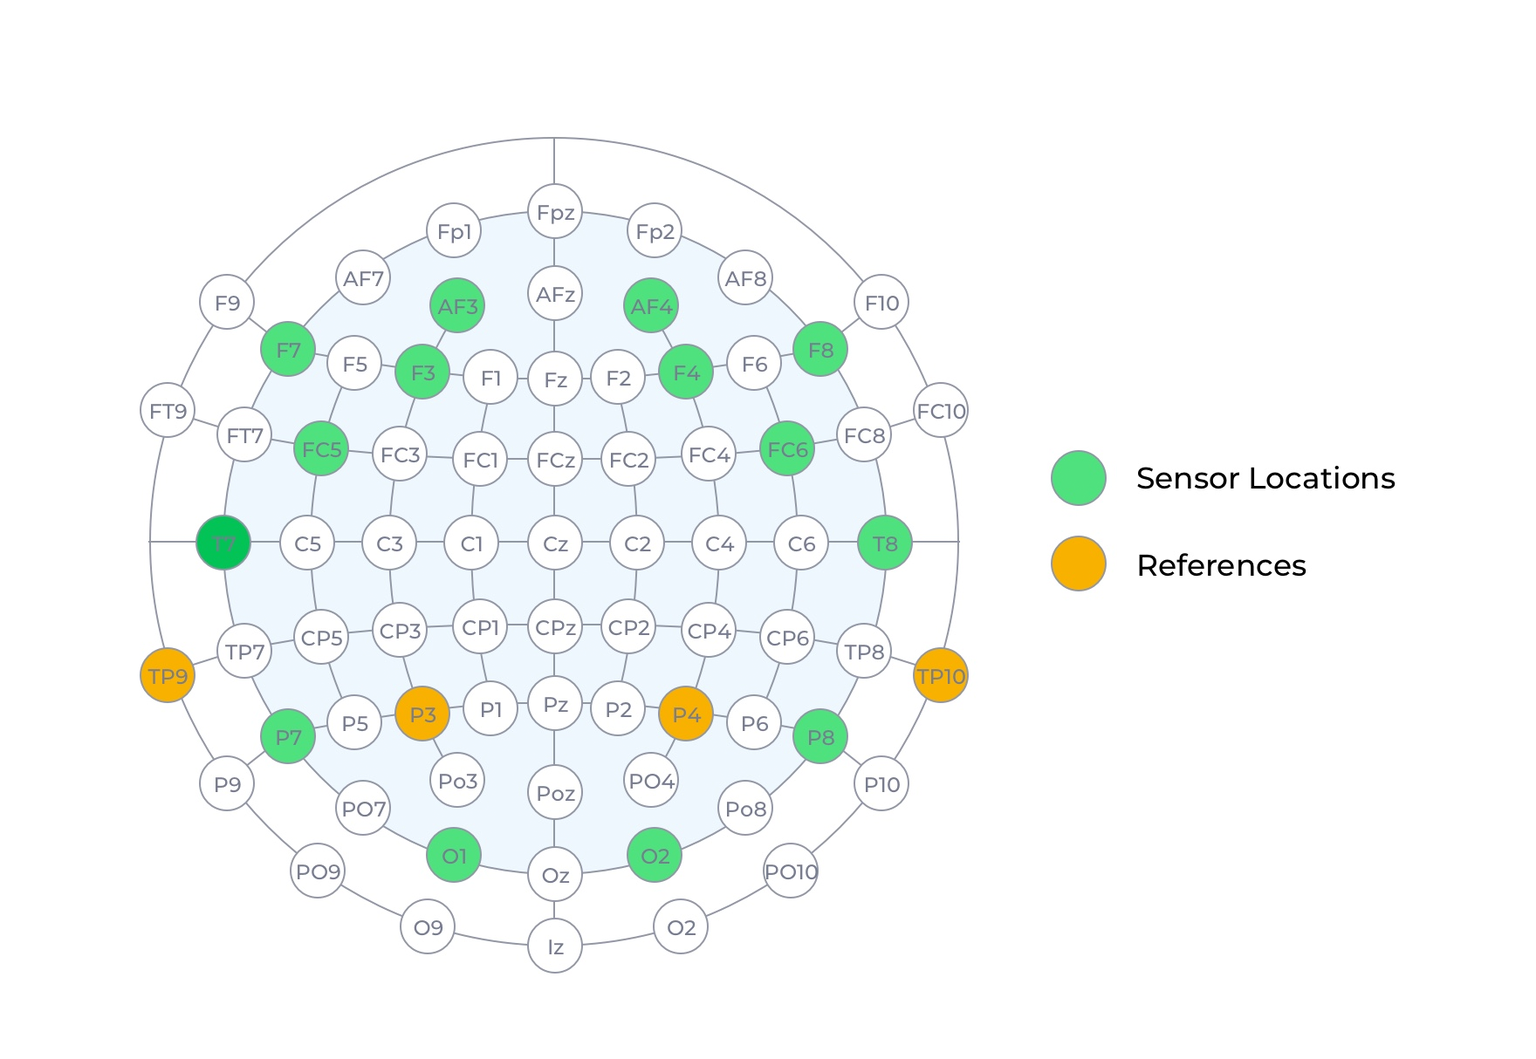
\includegraphics[width=0.85\linewidth]{Images/emotiv-epoc-x-mapping.png}
    \caption{Sensor locations of the Emotiv EPOC X mapped on the international 10--20 system}
    \label{fig:emotiv-epoc-x-mapping}
    \end{figure}

    \begin{figure}[H]
        \centering
        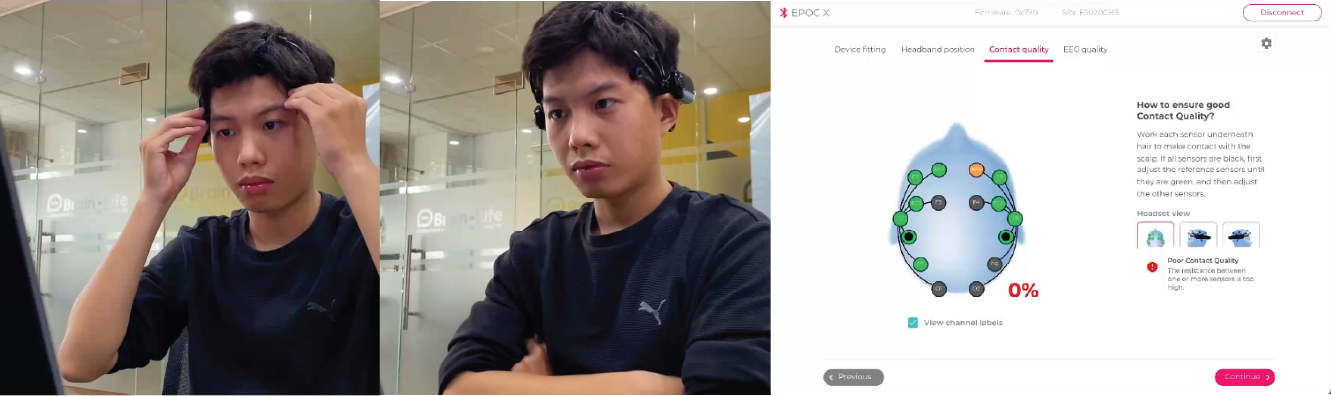
\includegraphics[width=\linewidth]{Images/epocx_wearing.png}
        \caption{Participant wearing the Emotiv EPOC X headset during data collection}
        \label{fig:epocx-wearing}
        \end{figure}

    % 5.2.2 Continuous EEG Data Streaming Architecture
    \subsection{Continuous EEG data streaming architecture}

    The data streaming architecture connects the physical headset to the software platform using a layered approach. This design ensures that the data collection process remains entirely separate from how each application mode utilizes the signals.

    At the hardware level, the Emotiv headset transmits raw EEG data over Bluetooth to the host computer. The official Emotiv Cortex desktop application receives this stream and exposes it through a local WebSocket at \texttt{wss://localhost:6868}. 
    
    This structure allows the project to access the brainwave data without needing to manage complex Bluetooth connections or low-level device drivers directly.

    Inside the platform, a dedicated background layer manages this local connection. It receives the continuous 128 Hz stream, discards unnecessary metadata such as stream counters, and extracts exactly 14 channel readings measured in microvolts ($\mu$V). This module acts as a central integration point. Whether the data originates from the real headset or a simulator, it is standardized into a steady stream of short, multi-channel arrays.



    To prevent this rapid 128 Hz influx from freezing the user interface, the integration layer uses a lightweight internal event system. Instead of adding heavy network routing between internal components, it pushes new samples to the active applications in the background. The three operational modes share this exact same streaming foundation but consume the data differently based on their specific needs:

    \begin{itemize}
    \item Graz Data Collection gathers EEG only during defined recording windows. It accumulates the samples internally and packages each window as a complete labeled trial for offline storage.

    \item Live MI Monitor consumes the stream continuously, feeding the incoming samples directly into the machine learning classifier for real-time predictions.

    \item Gamified Calibration routes the continuous EEG stream strictly to the backend Python game server to be held in a local memory buffer. The frontend browser game does not receive the heavy EEG stream for processing. Instead, it acts purely as an interactive controller, sending lightweight timing events, such as the start and end of a task, over the WebSocket during gameplay. The server uses these incoming events to mark accurate trial boundaries and extract the precise EEG segments from its internal buffer. During the real-time inference phase, the server processes the data and sends only the final classification results back to the browser for visual display.

    \end{itemize}

    \begin{figure}[H]
        \centering
        \setlength{\fboxsep}{10pt}
        \setlength{\fboxrule}{0.1pt}
        \fbox{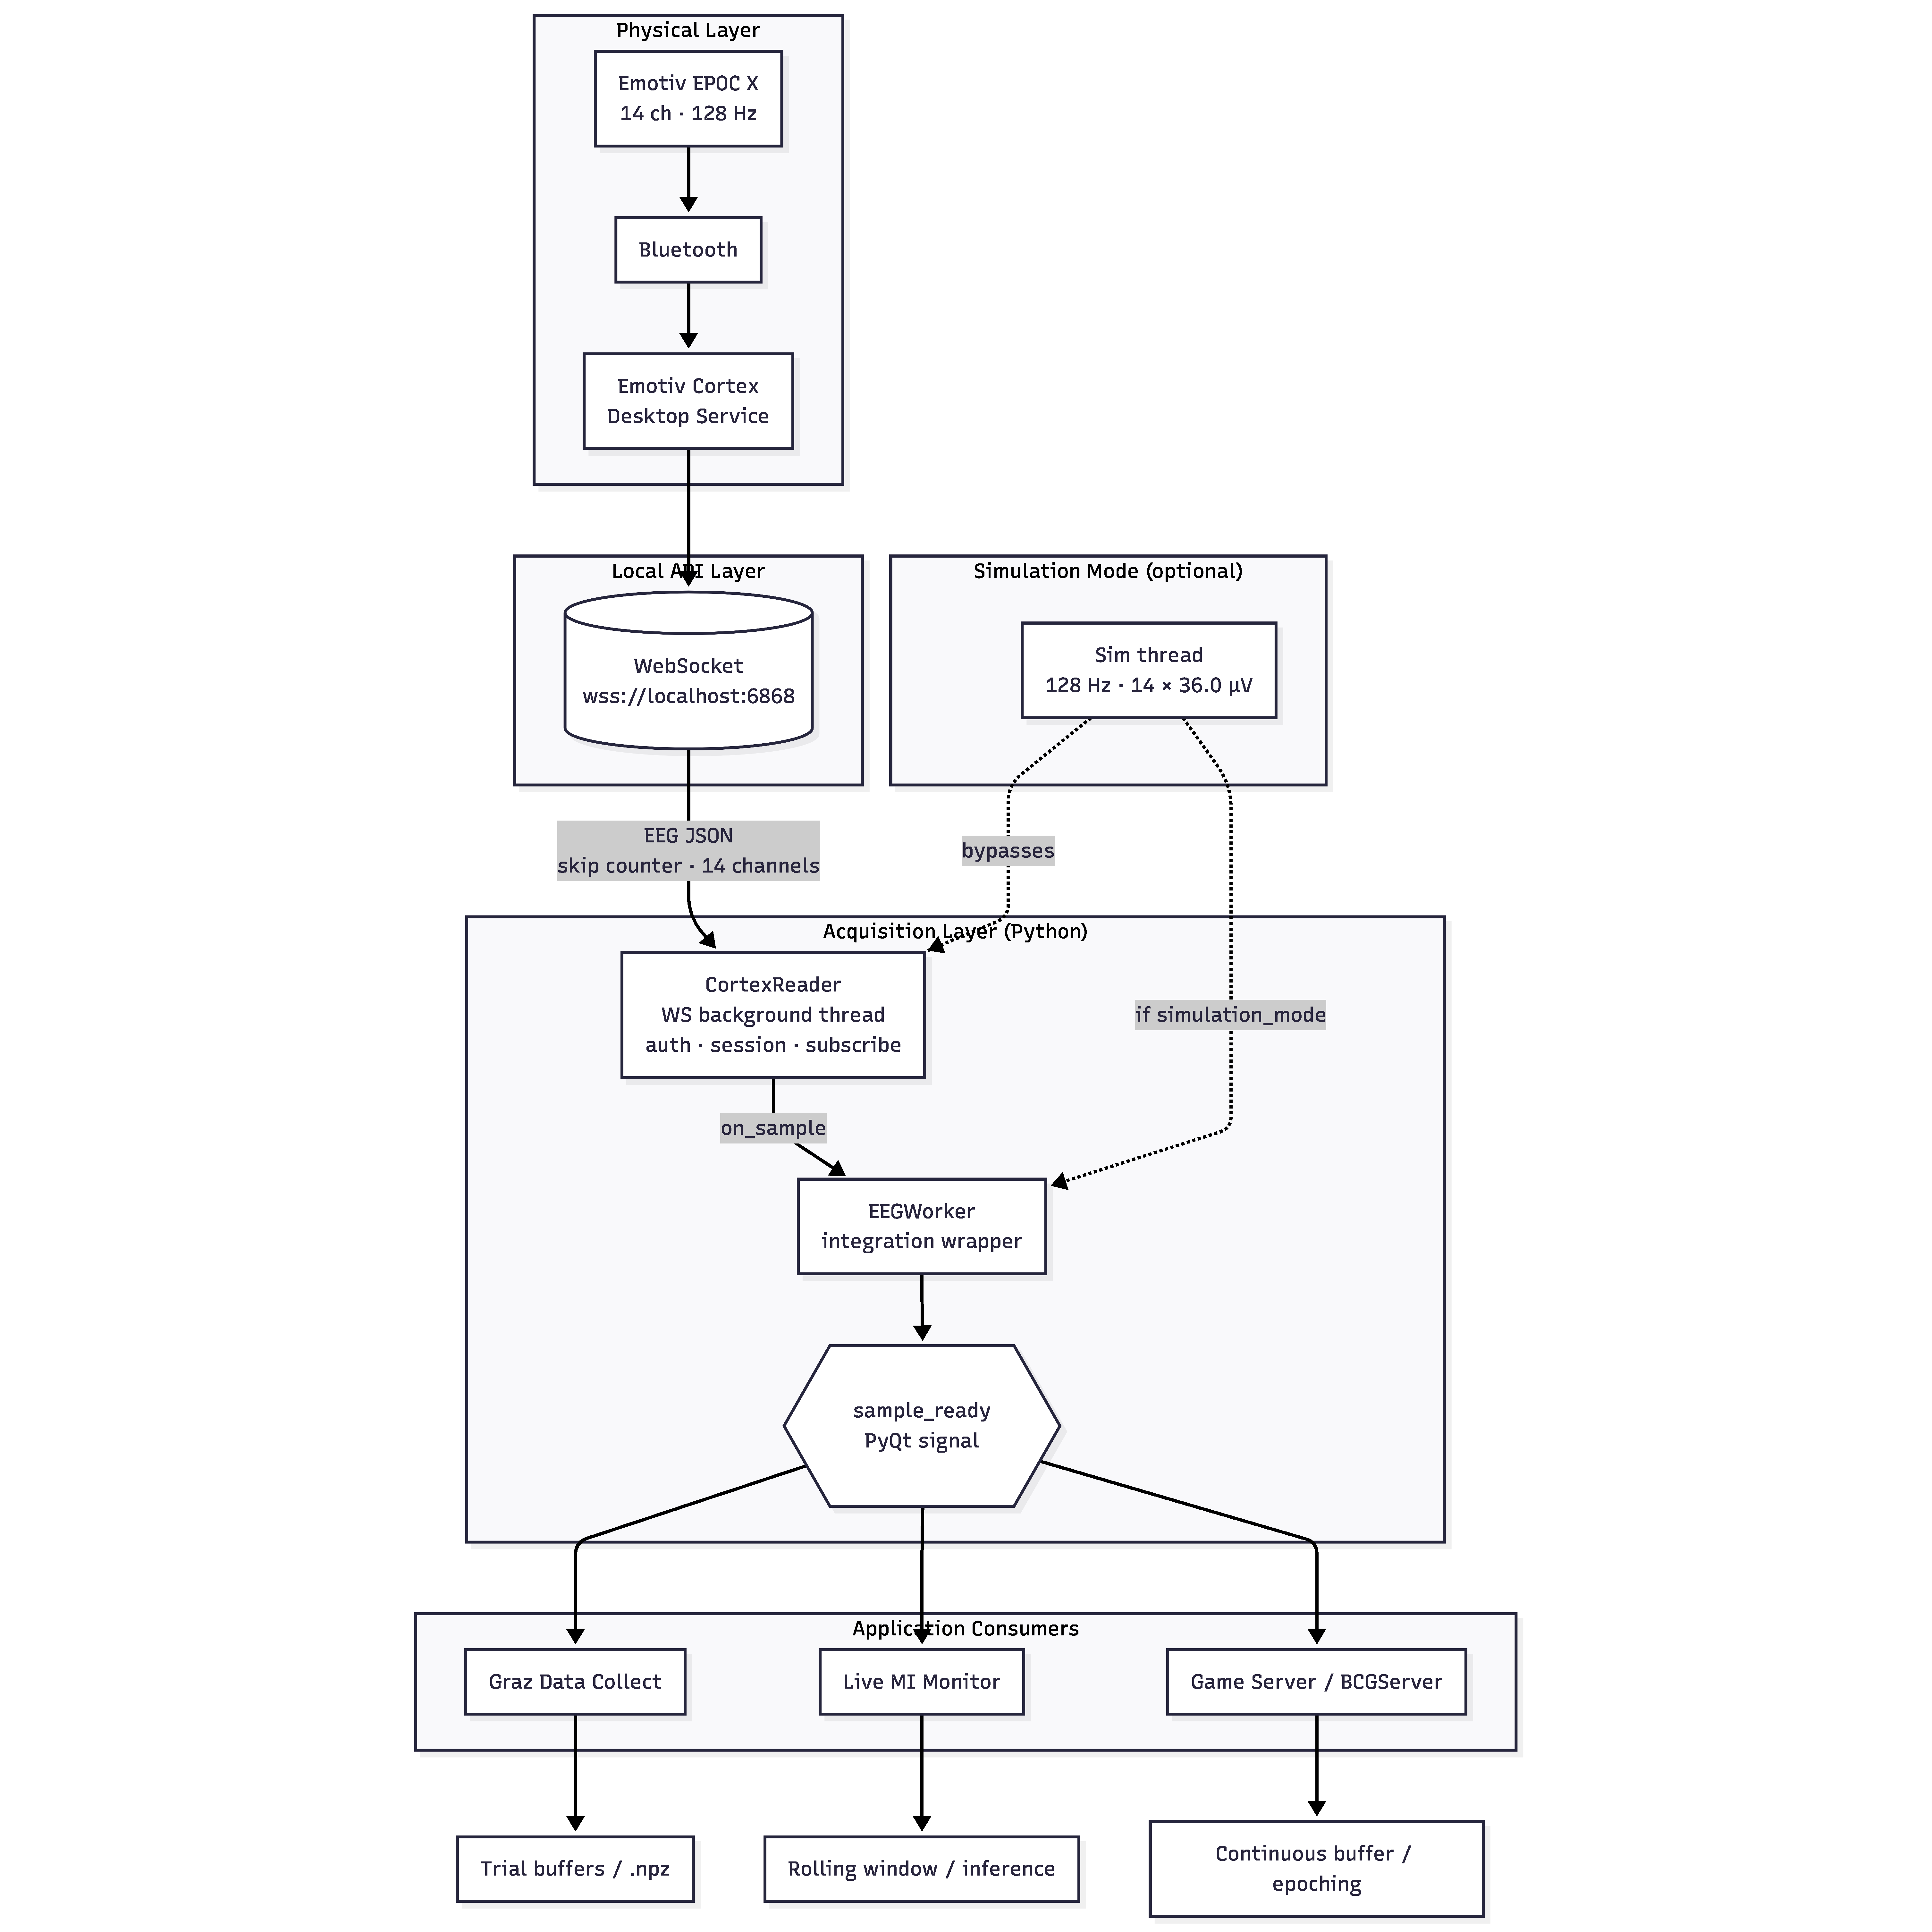
\includegraphics[width=0.8\textwidth]{Images/eeg-stream-flow.pdf}}
        \caption{Data flow diagram illustrating the multi layered acquisition pipeline from the Bluetooth headset through the Emotiv Cortex service and CortexReader module to the downstream UI components}
        \label{fig:data-flow-diagram}
        \end{figure}

    % 5.2.3 Hardware and signal simulation mechanisms
    \subsection{Hardware and signal simulation mechanisms}
    
    To enable hardware-independent testing, the platform supports two simulation modes: the official Emotiv 
    simulator for verifying API connectivity, and an internal 128 Hz mock stream generating fixed 14-channel 
    samples at 36.0 $\mu$V for validating data synchronization logic.
    

    % 5.3 Data Synchronization and Validation
    \section{Data synchronization and validation}

    % 5.3.1 Event Synchronization
    \subsection{Event synchronization}
    
    Linking a visual game event to the exact corresponding brainwave data is a primary technical challenge. Even though the browser game and the Python server run locally on the same machine, relying on system clocks or browser timestamps to cut the data is unreliable. Browser execution loops can experience slight delays (jitter) when rendering graphics, and the computer's system clock rarely synchronizes perfectly with the physical 128 Hz hardware sampling rate.

    To resolve this, the backend server uses a sample counting mechanism instead of time. It tracks a variable that increases by one for every single valid EEG sample received from the integration layer.

    When the browser game triggers an event, such as a note crossing the target line, it sends a lightweight JSON message over the WebSocket to mark the start of the task. The server instantly records the current sample count. When the 4.0-second task ends, the game sends another message, and the server records the new count. By using these two count markers, the server can accurately extract the exact block of EEG data. This anchors the gameplay strictly to the physical hardware stream, bypassing browser lag entirely.

    % 5.3.2 Data Validation and Output
    \subsection{Data validation and output}
    
    Before the collected data is saved or used for model training, it must pass a validation check to account for hardware instability. If the Bluetooth connection between the headset and the computer fluctuates, or if the background thread experiences buffering delays, some data samples might be lost.

    Since the system operates at a 128 Hz sampling rate, a standard 4.0-second task window must contain exactly 512 samples. The server counts the total collected samples within the designated boundaries. If this total falls below 80 percent of the expected length, the system assumes the data is corrupted and automatically discards the trial.

    If a trial passes this threshold but is slightly shorter or longer due to minor timing variations, the server applies an automatic padding or trimming algorithm. This forces every valid trial into a uniform multi-dimensional array shape of 14 channels by 512 samples. Once an entire gaming session is validated, the server saves the complete dataset locally as a compressed binary \texttt{.npz} file, making it immediately available for the machine learning pipeline.


    % 5.4 Machine Learning Implementation
    \section{Machine learning implementation}

    % 5.4.1 Signal Preprocessing
    \subsection{Signal preprocessing}
    
    Raw brainwave data contains significant noise that must be cleaned before any machine learning model can process it. The software applies a sequential filtering pipeline to isolate the relevant information.

    First, a bandpass filter is applied between 8 Hz and 30 Hz. This specific range is chosen because it isolates the Mu and Beta brain rhythms, which are the primary frequencies that react during motor imagery tasks. Next, a digital notch filter at 50 Hz is applied to remove background electrical interference caused by local power lines. Finally, the system normalizes the data across all 14 channels using a Z-score calculation to ensure the signal scale is consistent for the neural network.

    % 5.4.2 Transfer Learning Architecture
    \subsection{Transfer learning architecture}
    
    The system utilizes EEGNet, a compact Convolutional Neural Network designed specifically for brain signals \cite{lawhern2018eegnet}. However, training a deep neural network from scratch requires thousands of trials, which is impossible to collect in a short calibration session.

    To solve this, the project implements a transfer learning strategy. The model is first pre-trained offline using a large, public motor imagery dataset (BCI Competition IV 2a), which uses a 22-channel layout. Because the Emotiv EPOC X only has 14 channels, the model must be structurally adapted.

    The system loads the temporal layers from the pre-trained model and freezes them. These layers have already learned how to extract frequency patterns over time, which remains useful regardless of the hardware. However, the system discards the old spatial layers and reinitializes a new set of spatial weights designed specifically for the 14-channel layout. This hybrid approach allows the model to retain broad frequency knowledge while learning the user's specific spatial brain patterns during the short calibration game \cite{lawhern2018eegnet, giles2022transfer}.

    % 5.4.3 Session-Based Calibration Workflow
    \subsection{Session-based calibration workflow}
    
    The integration of the game and the machine learning model follows a three-stage lifecycle managed entirely on the backend server:

    Collection Phase: The server focuses strictly on recording, validating, and holding the incoming trials in its memory. The machine learning model remains inactive to save processing power.

    Calibration Phase: Once the game finishes and the data is validated, the server freezes the temporal layers and begins fine-tuning the new spatial layers using the newly collected user data. This produces a personalized model weight file saved locally.

    Inference Phase: The server transitions into real-time monitoring. It maintains a rolling buffer of the last 4.0 seconds of filtered data. Every 0.5 seconds, the customized model evaluates this buffer and sends the predicted user intention back to the browser interface.


    % 5.5 Game Interface Implementation
    \section{Game interface implementation}

    % 5.5.1 Game Loop and Timing
    \subsection{Game loop and timing}
    
    The frontend interface is a browser-based application built with the HTML5 Canvas API and JavaScript. Instead of performing heavy data processing, it functions purely as an interactive metronome to guide the user's mental tasks. The game loop operates continuously using the browser's native animation frames.

    A single calibration trial follows a strict timeline sequence. First, a visual note appears and travels down a lane for approximately 2.4 seconds, giving the user time to prepare. The moment the note reaches the hit line, the game sends the start event to the server, and the user holds their motor imagery focus for 4.0 seconds. This is immediately followed by a 0.5-second pause to allow the user to relax. The game then enters a 4.0-second neutral state to record the user's resting baseline brainwaves. Finally, another 0.5-second gap occurs before the next note spawns.

    % 5.5.2 Client-Server Communication
    \subsection{Client-server communication}
    
    The browser client controls session progression through JSON messages over WebSocket. Once the required 
    gameplay sequence is complete, the client issues a save command, and upon server confirmation, allows 
    the user to initiate backend calibration.


\chapter{System Results and Evaluation}

    % 6.1 Baseline Classifier Investigation
    \section{Baseline Classifier Investigation}
    
    As outlined in the project objectives, establishing a hardware-compatible baseline classifier is a prerequisite for a functional BCI system. To determine the most effective algorithm for the 14-channel Emotiv EPOC X, two distinct machine learning strategies were evaluated using established public datasets.

    % 6.1.1 Strategy 1: Classical Machine Learning
    \subsection{Strategy 1: Classical Machine Learning}
    
    The initial strategy evaluated the MIMED dataset, chosen because it was recorded using the same Emotiv EPOC X hardware utilized in this project. 
    
    The pipeline employed Common Spatial Pattern (CSP) for feature extraction, paired with classical classifiers such as Linear Discriminant Analysis (LDA) and Support Vector Machines (SVM) \cite{blankertz2008optimizing, lotte2018review}.

    However, the evaluation exposed a critical limitation: the MIMED dataset contains severe data scarcity, averaging only about eight trials per subject. This lack of data causes unstable CSP covariance estimation, leading to poor generalization on unseen data.

    \begin{table}[H]
        \centering
        \caption{Accuracy of Classical ML models on the 4-class MIMED dataset}
        \label{tab:classical-ml-results}
        \begin{tabular}{@{} l l l r @{}}
        \toprule
        \textbf{Model} & \textbf{Classes} & \textbf{Evaluation Protocol} & \textbf{Accuracy} \\
        \midrule
        CSP + LDA & 4-class & Cross-subject, 5-fold & 52.5\% \\
        CSP + SVM & 4-class & Cross-subject, 5-fold & 46.7\% \\
        CSP + LDA (Variant) & 4-class & Cross-subject, 5-fold & 42.1\% \\
        \bottomrule
        \end{tabular}
    \end{table}

    % 6.1.2 Strategy 2: Deep Learning and Transfer Learning
    \subsection{Strategy 2: Deep Learning and Transfer Learning}
    
    To overcome the data scarcity issue, the focus shifted to a deep learning approach utilizing the EEGNet architecture. To ensure the neural network learned general motor imagery characteristics (such as Mu and Beta rhythms), it was first pre-trained on the BCI Competition IV 2a dataset, a robust clinical dataset containing 5,184 trials across 9 subjects.

    Following this pre-training phase, the model was fine-tuned using the MIMED dataset. This transfer learning step adapted the general frequency patterns learned from the 22-channel dataset to the specific 14-channel spatial layout of the Emotiv EPOC X.

    \begin{table}[H]
        \centering
        \caption{Accuracy of EEGNet utilizing different training strategies}
        \label{tab:eegnet-results}
        \begin{tabular}{@{} p{0.4\textwidth} l l r @{}}
        \toprule
        \textbf{Model Configuration} & \textbf{Classes} & \textbf{Evaluation Protocol} & \textbf{Accuracy} \\
        \midrule
        EEGNet trained purely on BCI IV 2a & 4-class & 5-fold CV & 61.44\% \\
        EEGNet trained purely on MIMED & 2-class & LOTO & 71.67\% \\
        EEGNet pre-trained on BCI IV 2a, fine-tuned on MIMED & 2-class & LOTO & 72.08\% \\
        \bottomrule
        \end{tabular}
    \end{table}

    The results demonstrate that pre-training the network prior to fine-tuning it on target hardware yields 
    the highest accuracy (72.08\%) on the MIMED public dataset. This offline evaluation on publicly available 
    data establishes the technical feasibility of the transfer learning approach for 14-channel hardware. While 
    this accuracy was achieved on existing datasets rather than user-collected data from the BCG system, it 
    provides a methodological foundation for the architectural design of the adaptive pipeline.


    % 6.2 System Interface and Pipeline Validation
    \section{System Interface and Pipeline Validation}

    During inference testing with simulated data, the backend pipeline consistently processed 512-sample EEG 
    segments and returned classification results within the required 0.5-second window.

    \begin{figure}[H]
        \centering
        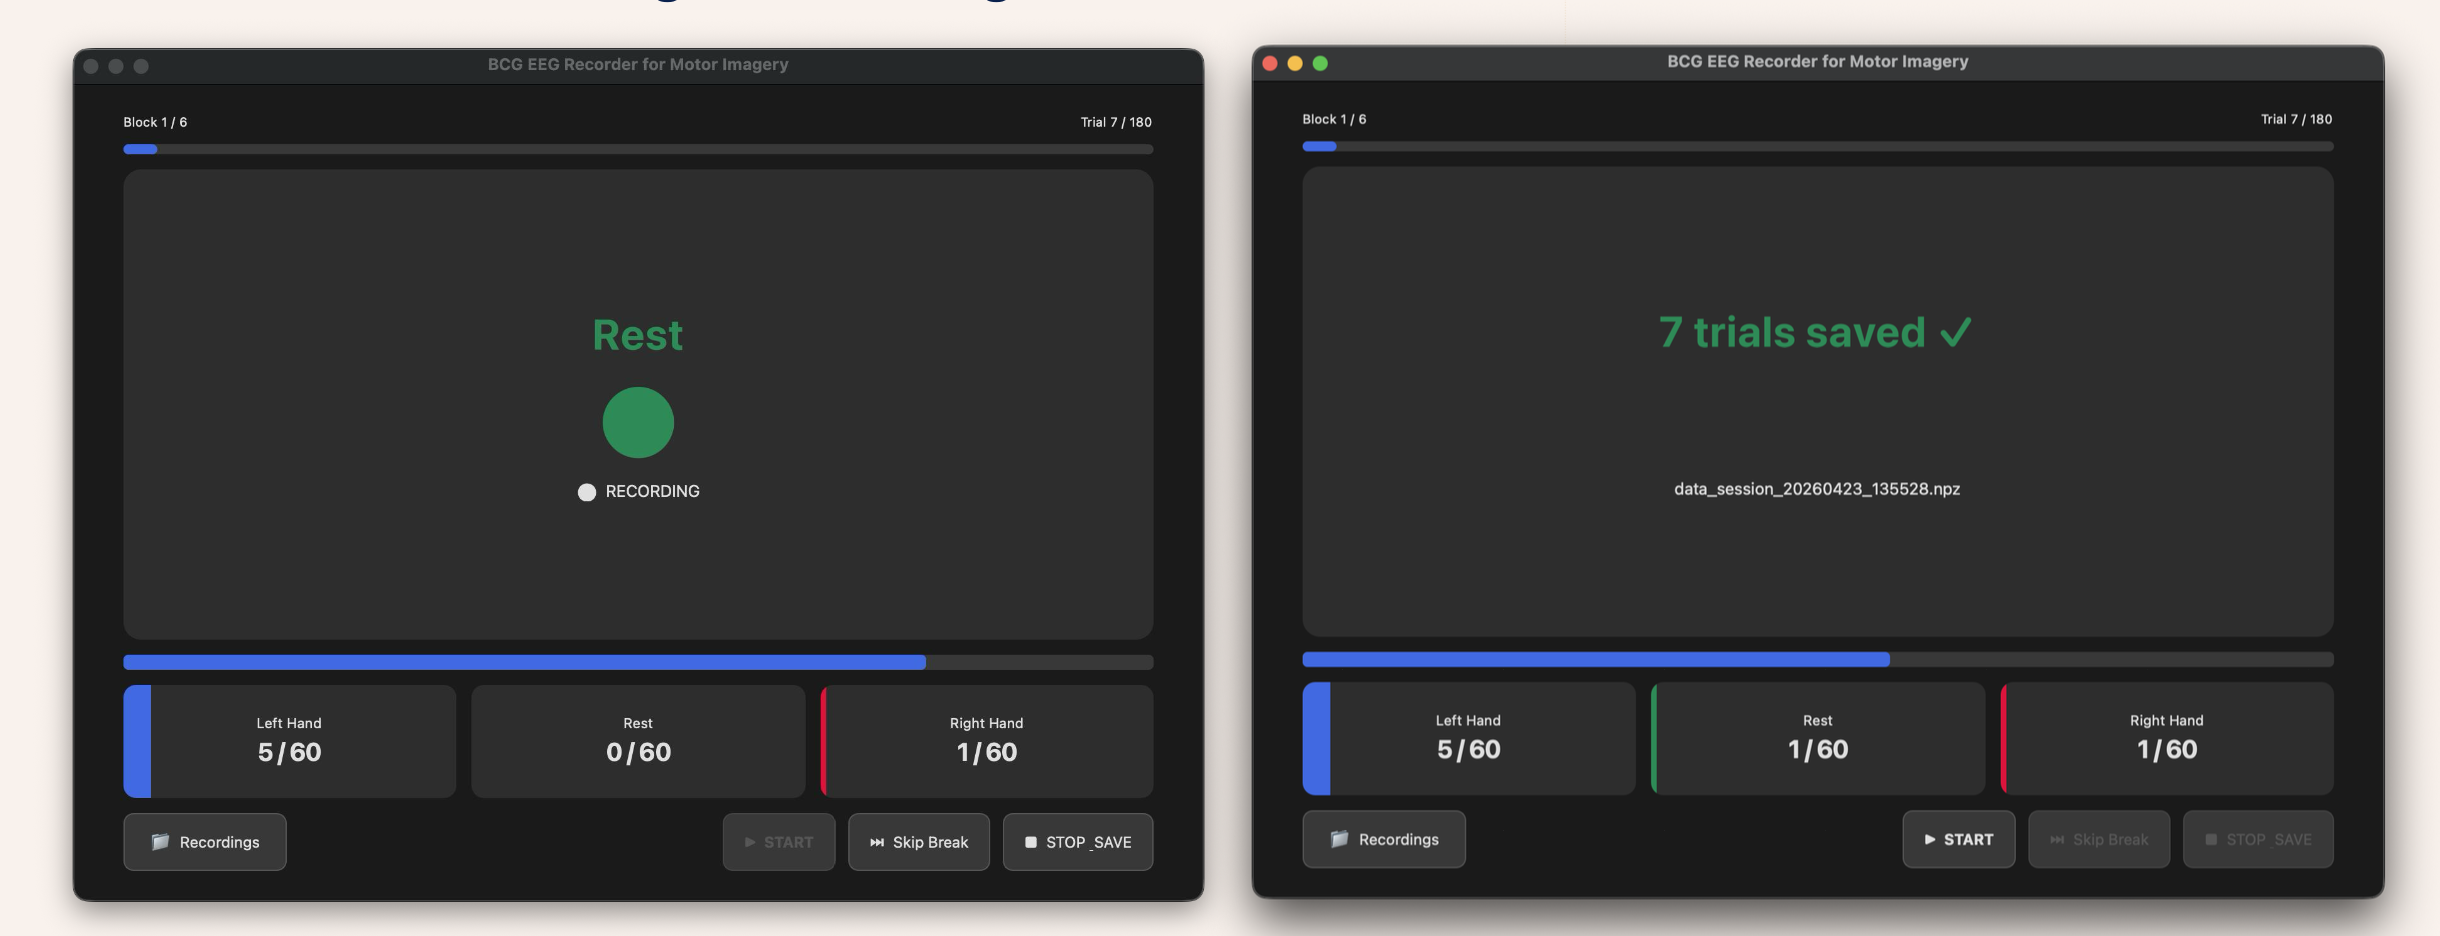
\includegraphics[width=0.85\textwidth]{Images/graz-interface.png}
        \caption{The standard Graz Data Collect interface used for the baseline condition}
        \label{fig:graz-interface}
    \end{figure}

    \begin{figure}[H]
        \centering
        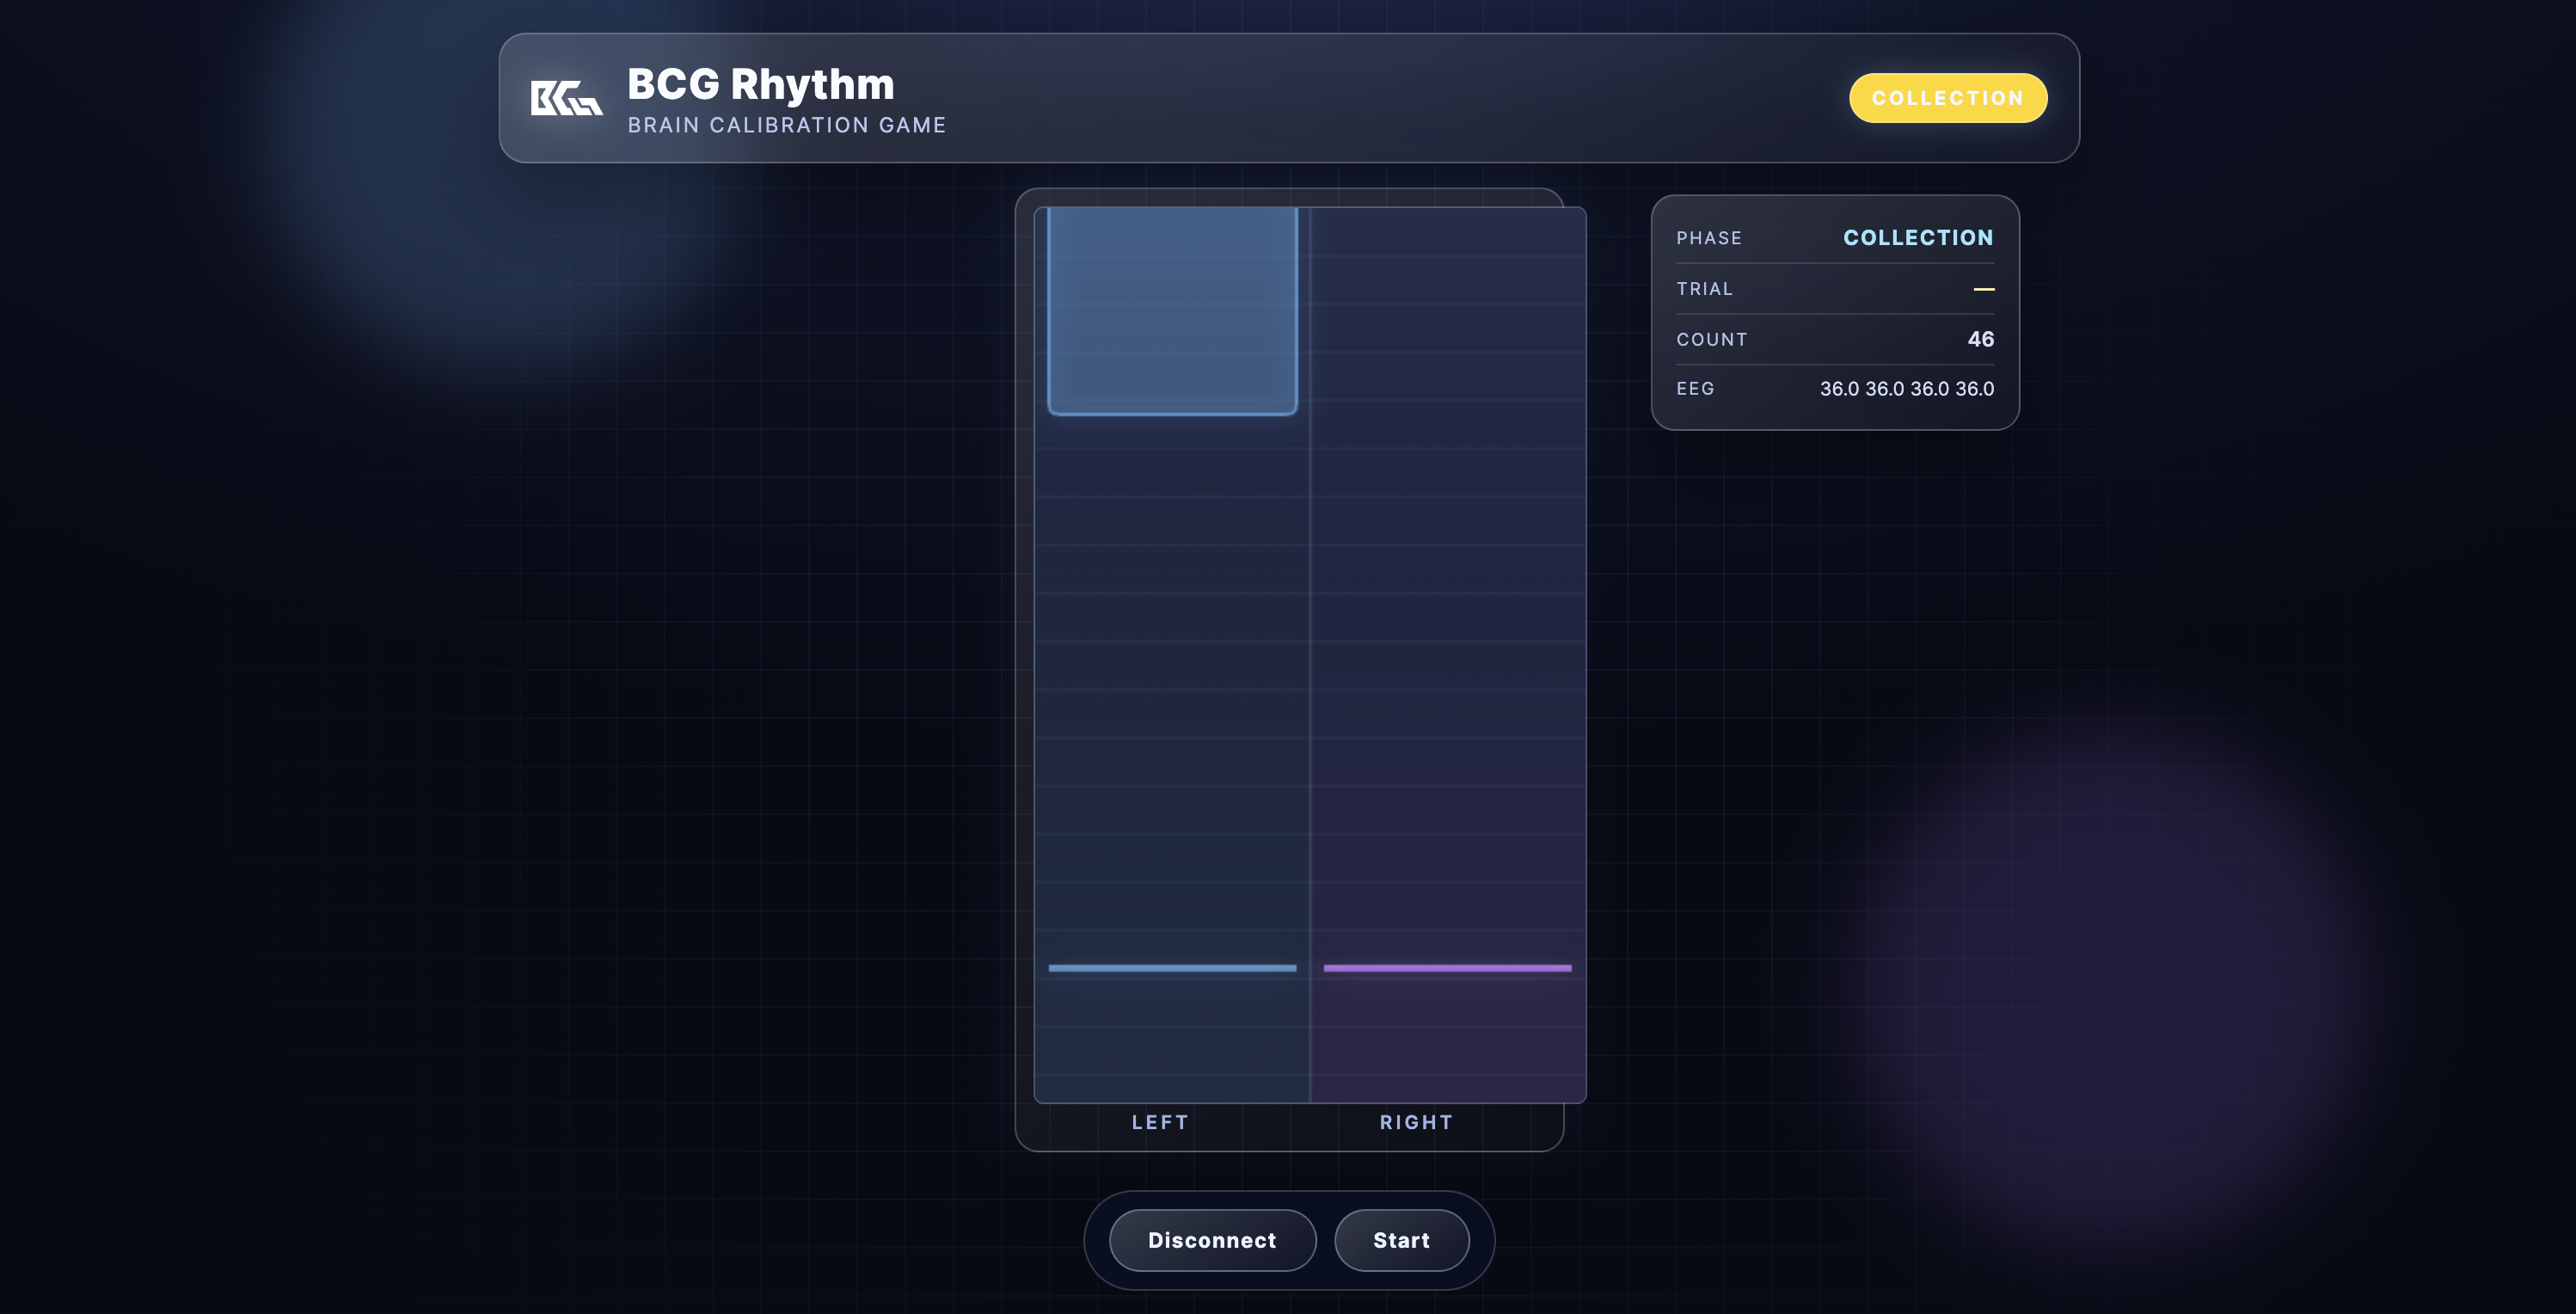
\includegraphics[width=0.85\textwidth]{Images/game-interface.png}
        \caption{The Gamified Calibration interface utilizing covert cues during gameplay}
        \label{fig:game-interface}
    \end{figure}

    \begin{figure}[H]
        \centering
        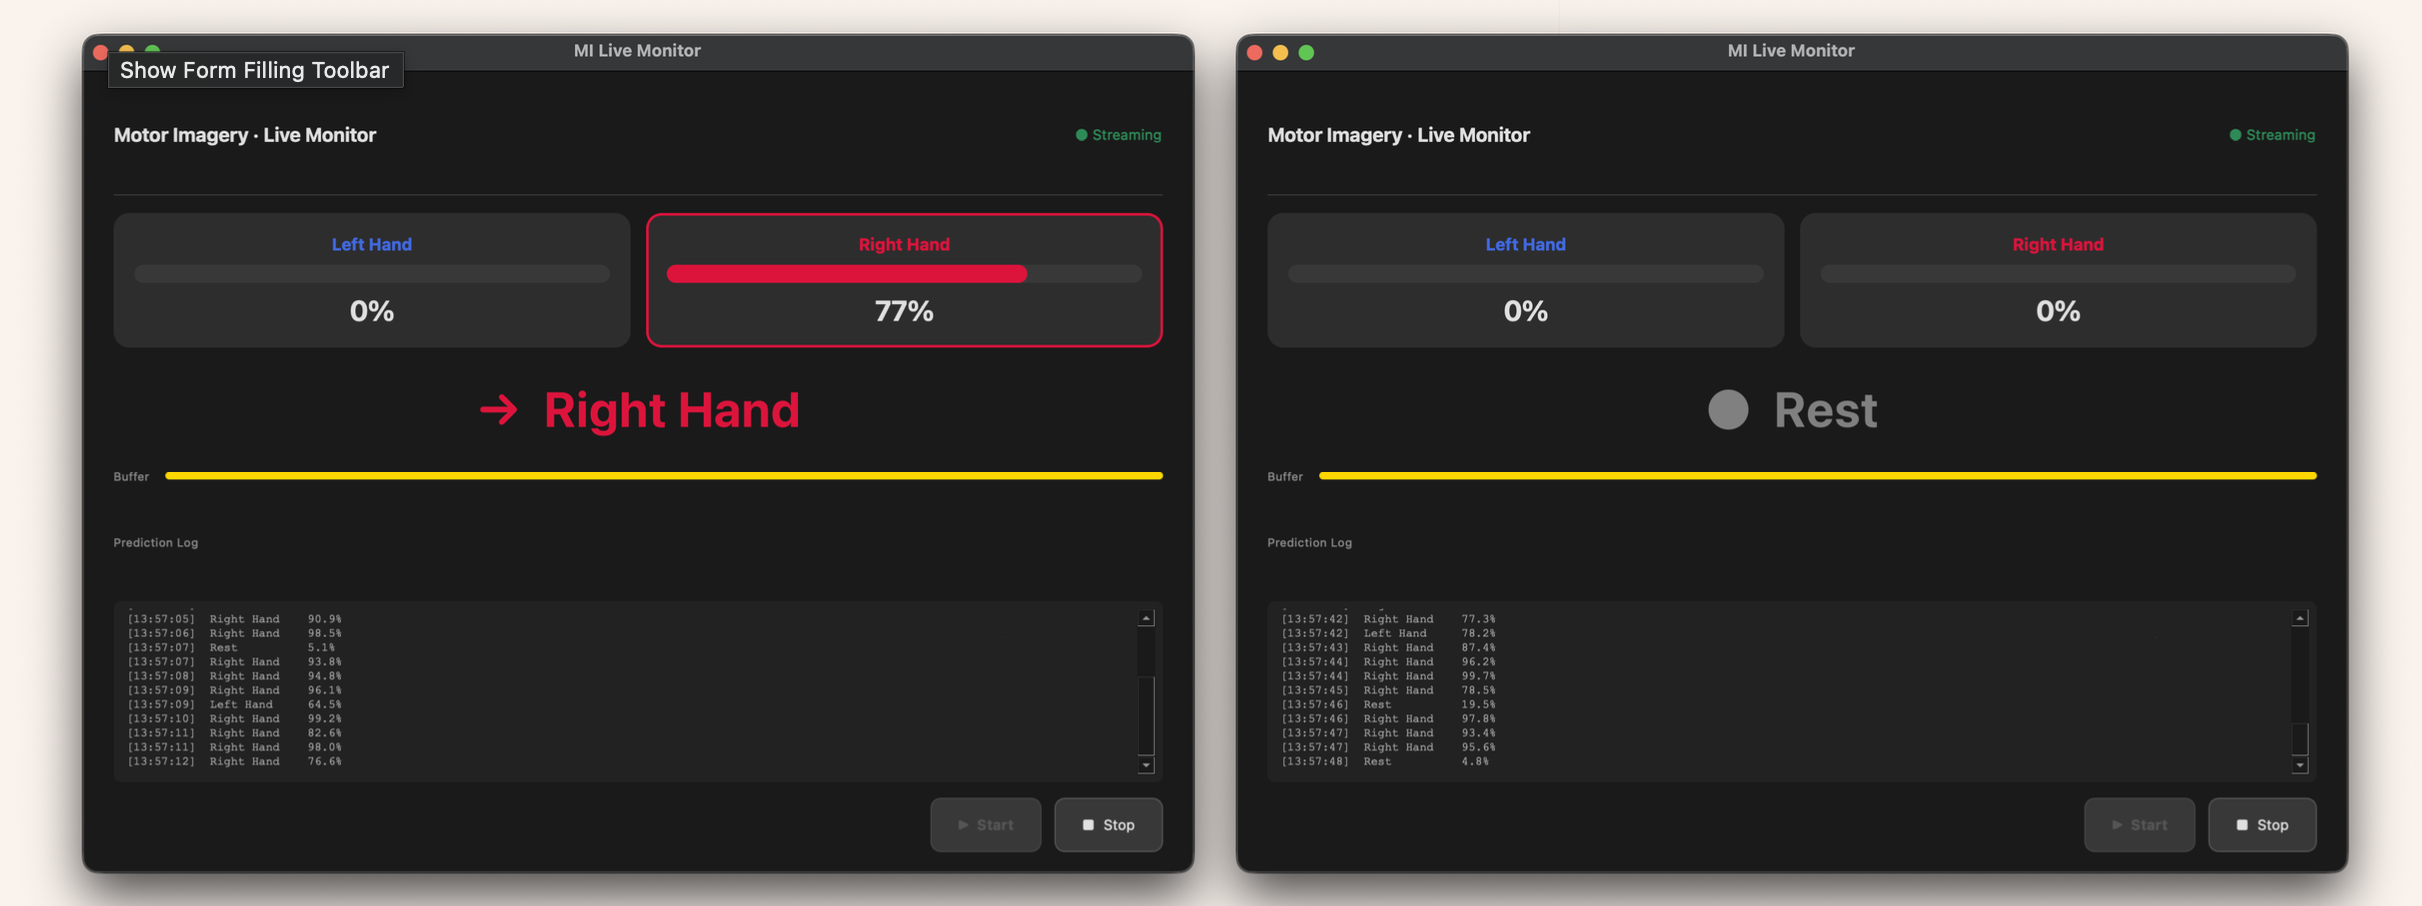
\includegraphics[width=0.85\textwidth]{Images/inference-interface.png}
        \caption{The Live MI Monitor interface displaying real-time classification results}
        \label{fig:inference-interface}
    \end{figure}


    % 6.3 User Study: Workload and Experience
    \section{User Study: Workload and Experience}

    % 6.3.1 Study Setup and Methodological Adjustments
    \subsection{Study Setup and Methodological Adjustments}
    
    To evaluate the effectiveness of the gamified approach, a between-subjects user study was conducted. Ten healthy participants were equally divided into two groups: five utilizing the traditional Graz protocol and five utilizing the Gamified protocol.

    Shortly prior to the deployment of the user study, a serialization issue within the internal data buffering module was identified, which occasionally corrupted the saved \texttt{.npz} arrays. Due to this technical constraint and the limited project timeline, the evaluation was refocused solely on the Human-Computer Interaction (HCI) aspect through NASA-TLX assessment. Participants completed the full 10-minute calibration tasks under realistic conditions, but the raw EEG data was not written to disk. This methodological adjustment allowed for a controlled comparison of the subjective workload between the two interface designs, though it prevents direct validation of signal quality differences between the protocols.

    % 6.3.2 Subjective Workload Results (NASA-TLX)
    \subsection{Subjective Workload Results (NASA-TLX)}
    
    Immediately following the calibration sessions, participants completed the NASA-TLX questionnaire to assess their perceived workload. Responses were recorded on a scale from 0 to 10 (where 0 indicates low demand or perfect performance, and 10 indicates high demand or failure). The results, averaged across the five participants in each group, are presented in Table 6.3.

    \begin{table}[H]
        \centering
        \caption{Average NASA-TLX workload scores comparing the Graz and Gamified protocols (N=5 per condition, scale 0--10)}
        \label{tab:nasa-tlx-results}
        \begin{tabular}{@{} l c c @{}}
        \toprule
        \textbf{NASA-TLX Dimension} & \textbf{Graz Protocol} & \textbf{Gamified Protocol} \\
        & \textbf{(Average)} & \textbf{(Average)} \\
        \midrule
        Mental Demand & 7.8 & 6.0 \\
        Physical Demand & 2.6 & 2.0 \\
        Temporal Demand & 4.0 & 2.6 \\
        Performance & 3.8 & 3.0 \\
        Effort & 7.6 & 4.2 \\
        Frustration & 5.4 & 3.2 \\
        \bottomrule
        \end{tabular}
    \end{table}

    To provide a comprehensive view of the cognitive footprint across all dimensions, Figure 6.4 maps the workload results on a radar chart.

    \begin{figure}[H]
        \centering
        \setlength{\fboxsep}{10pt}
        \setlength{\fboxrule}{0.1pt}
        \fbox{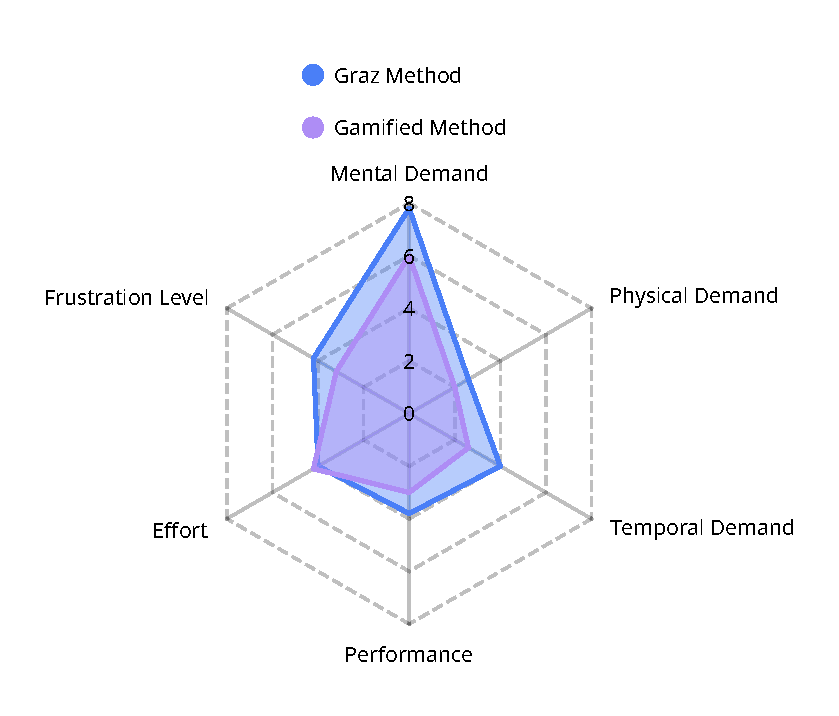
\includegraphics[width=0.7\textwidth]{Images/user-study-radar-chart.pdf}}
        \caption{Radar chart mapping the multi-dimensional workload footprint of the Graz vs. Gamified protocols}
        \label{fig:nasa-tlx-radar}
    \end{figure}

    The data reveals a reduction in perceived cognitive burden when utilizing the gamified environment. The most notable 
    difference is observed in the Effort category, which dropped from an average of 7.6 in the Graz protocol to 4.2 in 
    the gamified system. Furthermore, Frustration levels decreased from 5.4 to 3.2, and Mental Demand dropped from 7.8 
    to 6.0. Interestingly, despite the reduced reported effort, participants in the gamified group perceived their 
    Performance to be better (3.0) compared to the Graz group (3.8). These preliminary findings suggest that the game-based 
    interface may reduce the perceived repetitiveness of the calibration task, though the small sample size (N=5 per group) 
    and absence of recorded EEG data limit the scope of interpretation to subjective workload measures only.


\chapter{Conclusion}

    % 7.1 Project Summary and Key Findings
    \section{Project Summary and Key Findings}

    % 7.1.1 Resolution of the Calibration Bottleneck
    \subsection{Resolution of the Calibration Bottleneck}
    
    This project addressed the cognitive fatigue associated with traditional BCI calibration through a game-based 
    interface design. By embedding task cues within a rhythm game, the system demonstrated that the calibration 
    process can be redesigned to reduce perceived workload, as evidenced by NASA-TLX measures, without relying 
    on explicit directional prompts.

    % 7.1.2 Technical and Algorithmic Outcomes
    \subsection{Technical and Algorithmic Outcomes}
    
    The project delivered a dual-mode software architecture that integrated the Emotiv EPOC X headset and managed 
    128 Hz data streaming. Utilizing an EEGNet transfer learning pipeline (pre-trained on BCI IV 2a and fine-tuned 
    on MIMED), offline evaluation on public datasets achieved a baseline accuracy of 72.08\%, establishing the 
    technical viability of transfer learning for 14-channel hardware in limited-data scenarios.

    % 7.1.3 HCI and Workload Evaluation
    \subsection{HCI and Workload Evaluation}
    
    The comparative NASA-TLX evaluation (N=10, five per condition) indicated a reduction in perceived cognitive 
    workload for the gamified interface. Most notably, reported Effort dropped by 44\% (from 7.6 to 4.2), and 
    Frustration decreased from 5.4 to 3.2. These preliminary findings suggest that gamification may offer a 
    promising direction for optimizing the user experience during the calibration procedure, though further 
    studies with larger sample sizes and physiological signal validation would be needed to generalize these results.


    % 7.2 Limitations
    \section{Limitations}

    % 7.2.1 Incomplete Adaptive Pipeline
    \subsection{Incomplete Adaptive Pipeline}
    
    Due to time constraints, the adaptive fine-tuning mechanism remains at 
    the design and architectural stage. While the transfer learning pipeline has been validated on public datasets, 
    the integration for real-time model personalization and inference has not been fully implemented or tested with 
    user-collected data from the gamified calibration sessions.

    % 7.2.2 Sample Size and Demographics
    \subsection{Sample Size and Demographics}
    
    The evaluation was limited to 10 healthy participants, which does not fully 
    reflect the cognitive and physical realities of the target demographic: individuals with severe motor disabilities.

    % 7.2.3 Absence of Signal Quality Validation
    \subsection{Absence of Signal Quality Validation}
    
    Due to the data serialization issue encountered during the user study, 
    the project was unable to compare EEG signal quality between the Graz and gamified protocols. Consequently, the 
    evaluation is restricted to subjective workload measures (NASA-TLX) and cannot directly assess whether the game-based 
    interface produces MI signals of comparable fidelity to the standard protocol.


    % 7.3 Future Work
    \section{Future Work}

    % 7.3.1 Data Persistence and Pipeline Completion
    \subsection{Data Persistence and Pipeline Completion}
    
    The immediate technical priority is resolving the data 
    serialization bug to enable reliable storage of user-collected EEG data. Following this fix, the adaptive 
    fine-tuning mechanism should be fully implemented and integrated to complete the end-to-end pipeline: 
    gamified data collection, automated model calibration, and real-time inference feedback within the same session.

    % 7.3.2 Signal Quality Validation
    \subsection{Signal Quality Validation}
    
    Conduct a comparative study with functional data persistence to directly 
    assess whether EEG signals collected via the gamified protocol exhibit equivalent quality and discriminability 
    to those obtained through the standard Graz protocol. This validation is essential to substantiate the claim 
    that covert-cue approaches maintain signal fidelity.

    % 7.3.3 Extended User Studies
    \subsection{Extended User Studies}
    
    Expand the evaluation to include larger sample sizes and, critically, participants 
    from the target demographic (individuals with motor impairments) to assess ecological validity and real-world 
    applicability of the gamified calibration approach.

\chapter{Appendices}
    \section{Appendix A: Project timeline}

    \begin{figure}[H]
        \centering
        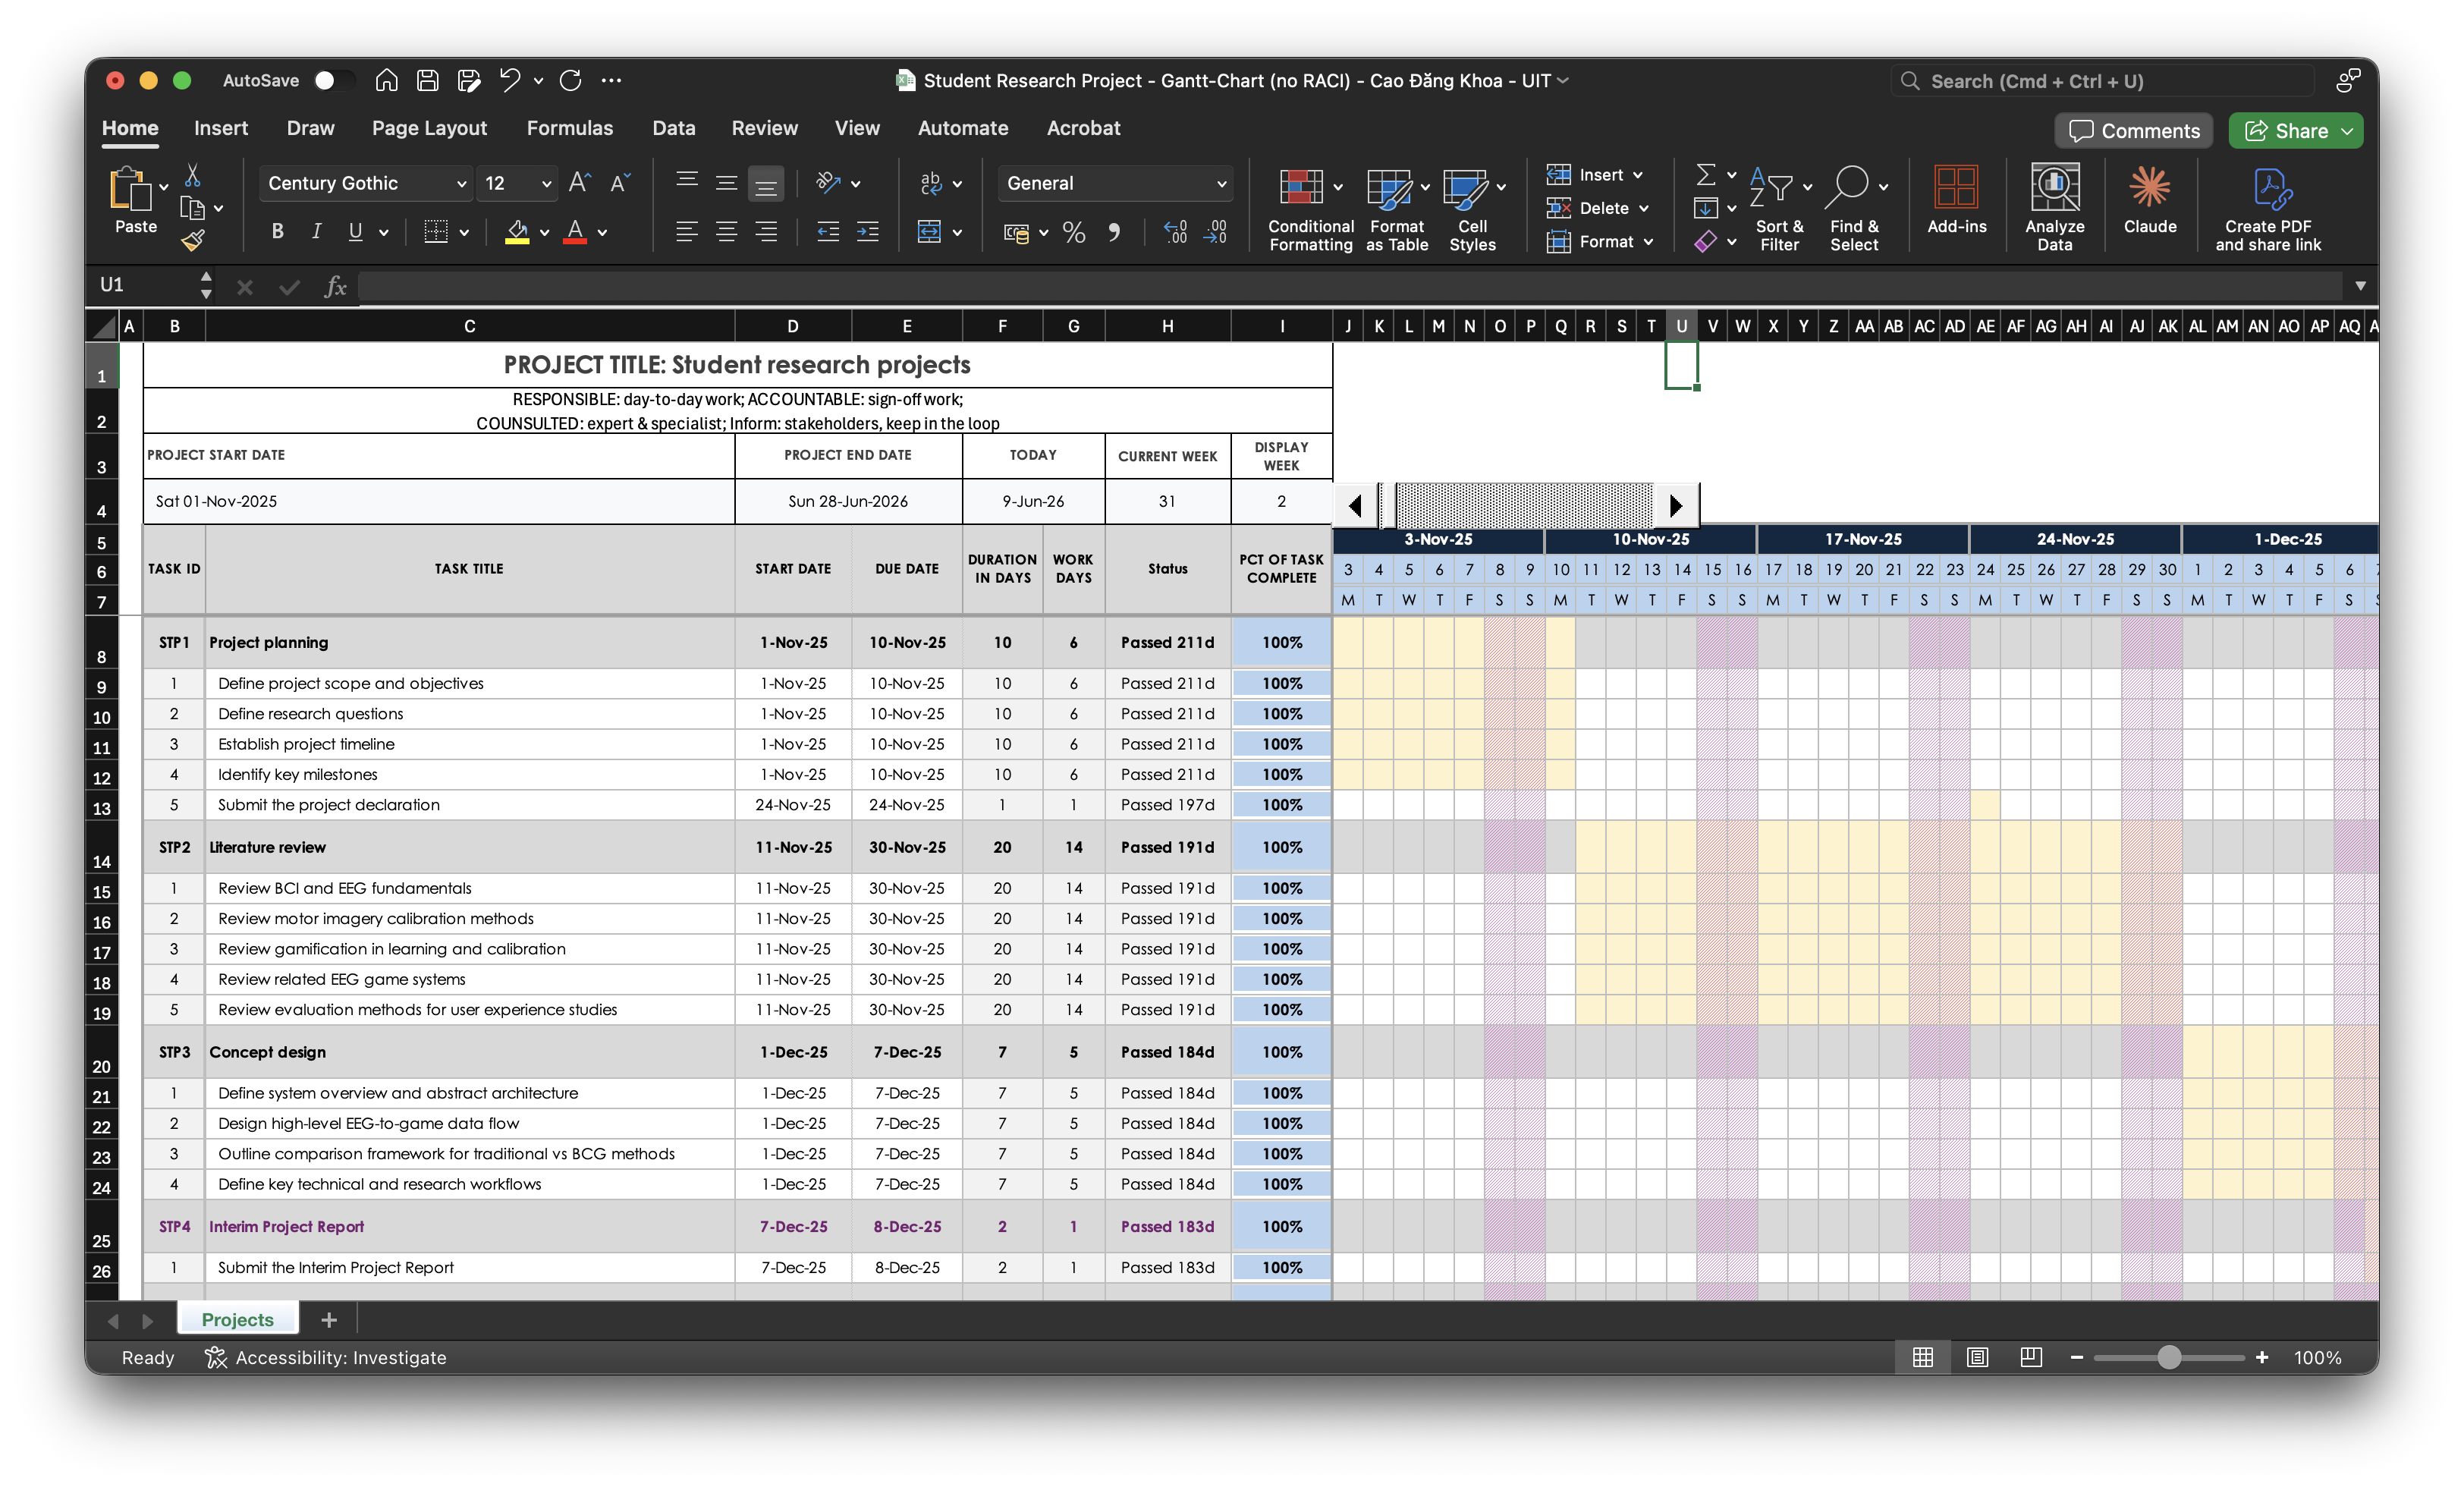
\includegraphics[width=1\textwidth]{Images/gantt-chart-new-1.png}
        \caption{Project Timeline - Part 1}
        \label{fig:gantt-chart-part-1}
    \end{figure}

    \begin{figure}[H]
        \centering
        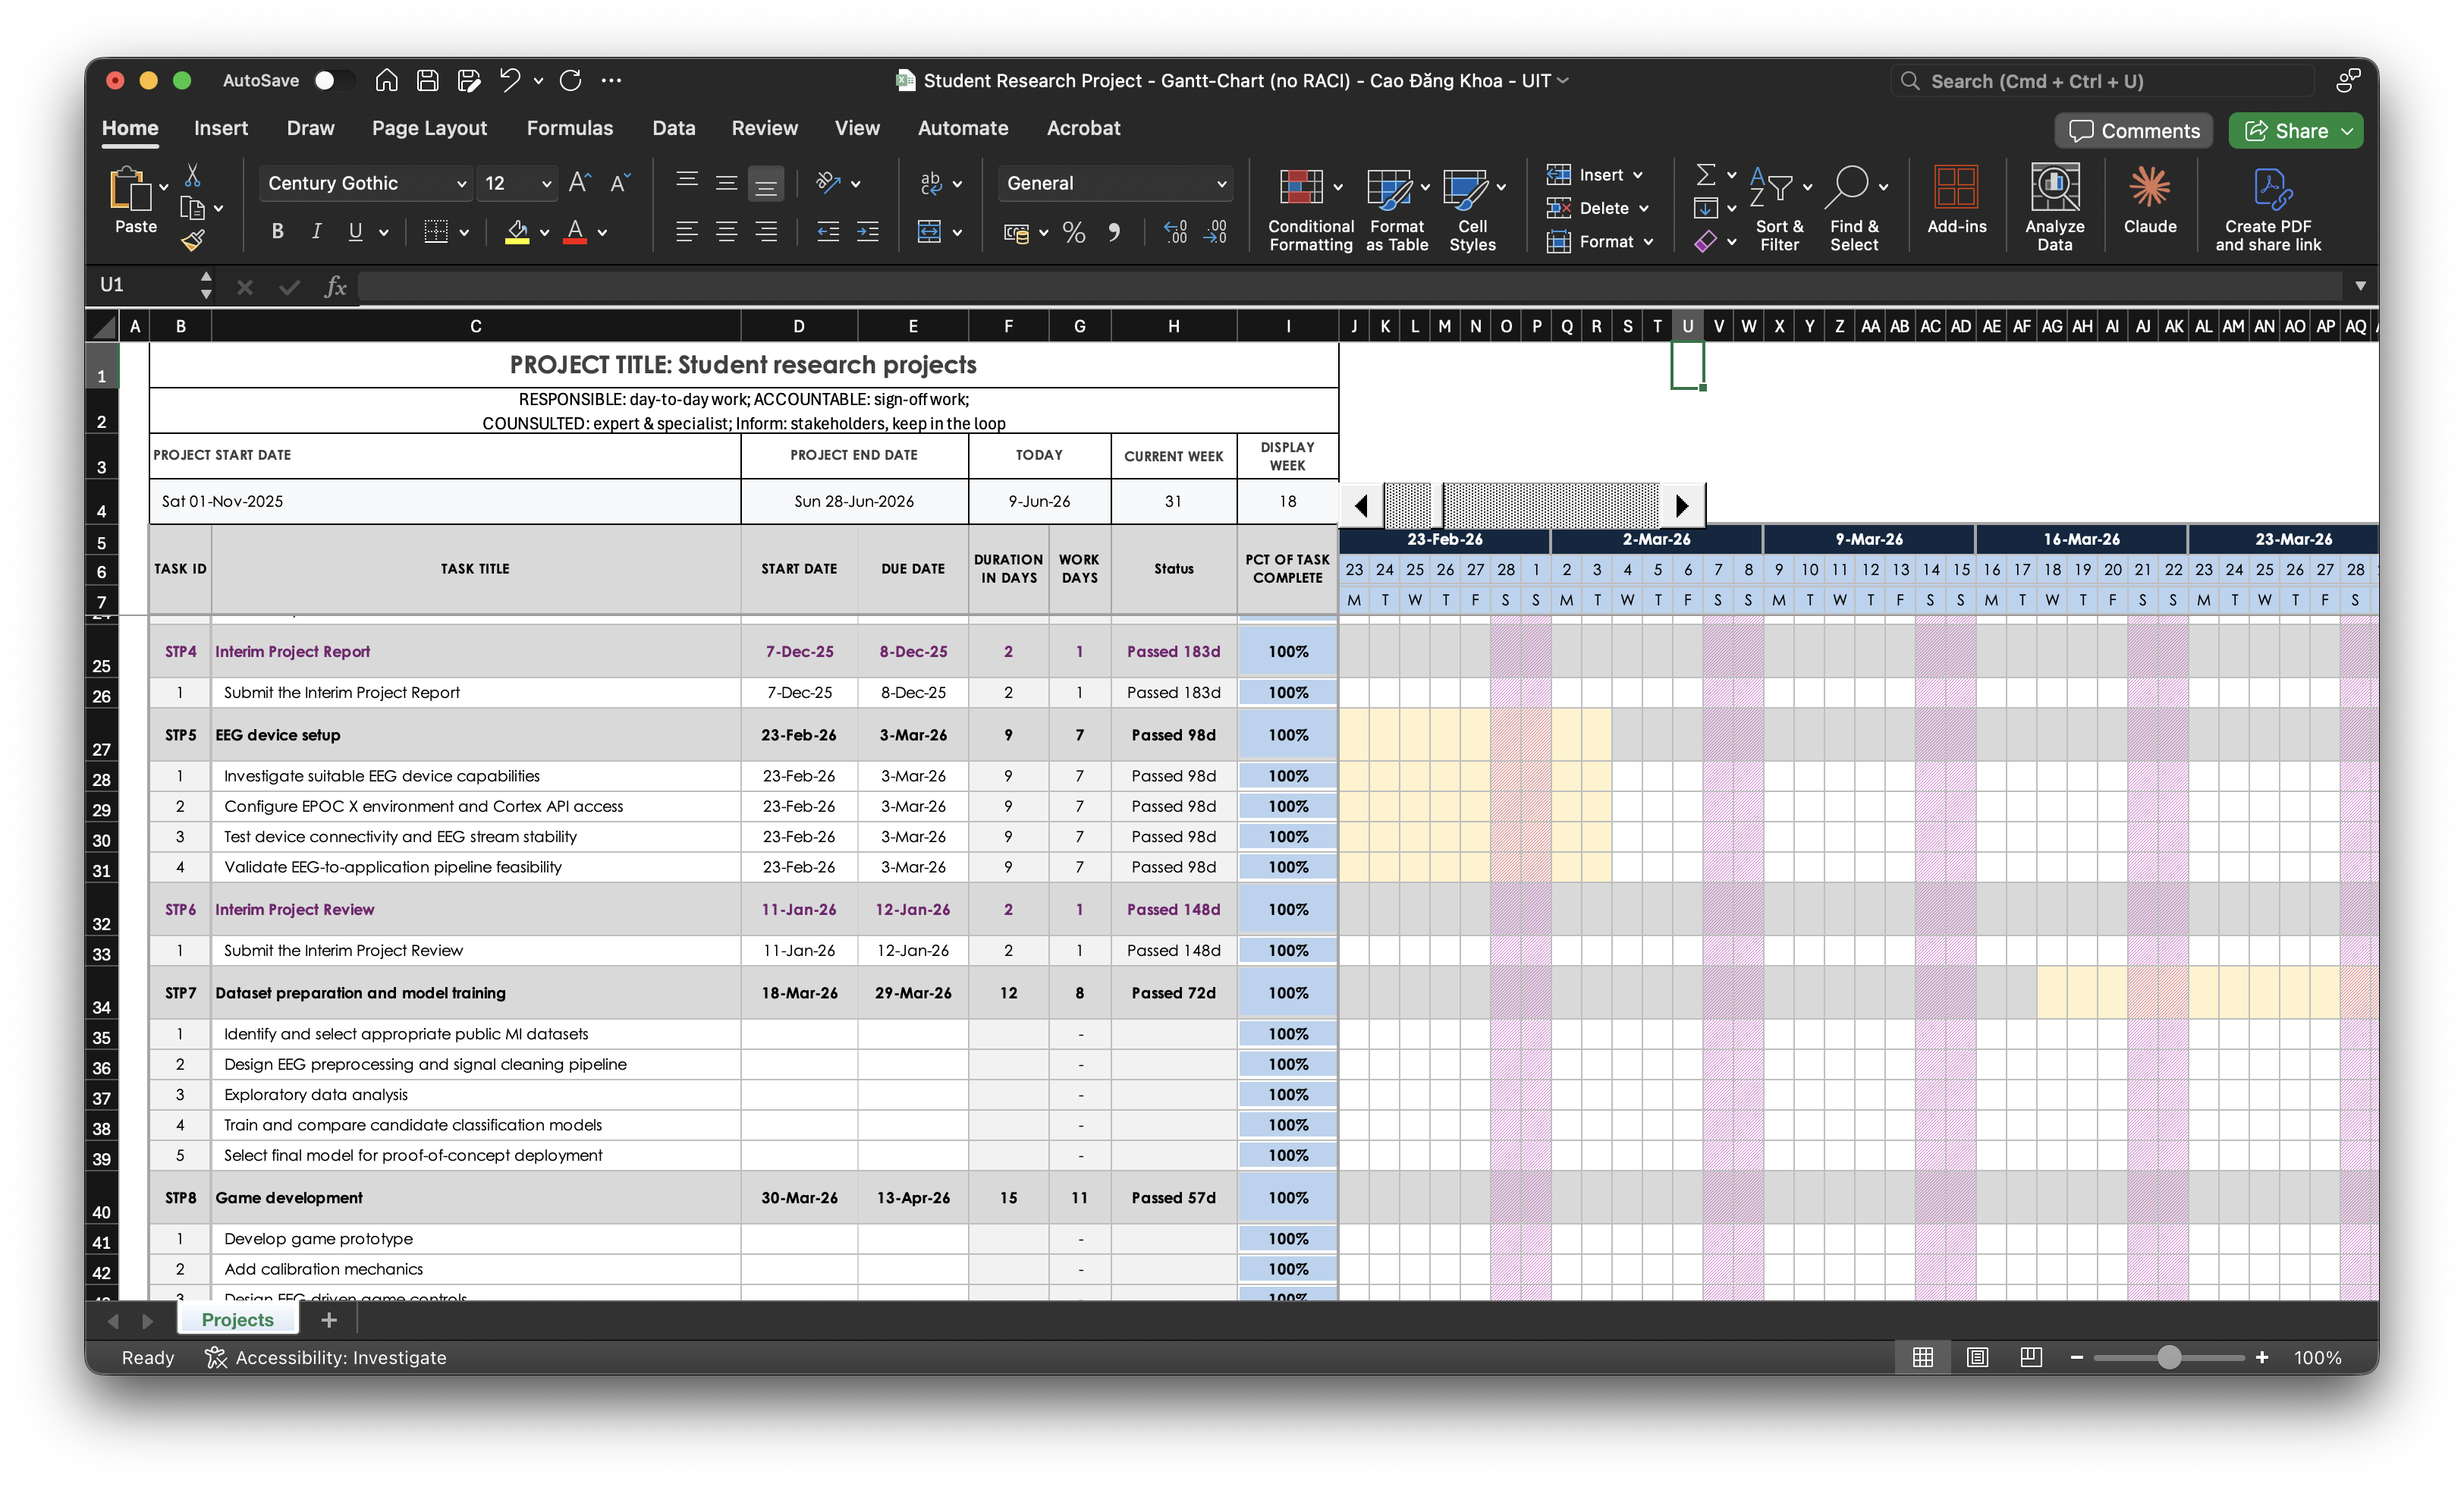
\includegraphics[width=1\textwidth]{Images/gantt-chart-new-2.png}
        \caption{Project Timeline - Part 2}
        \label{fig:gantt-chart-part-2}
    \end{figure}

    \begin{figure}[H]
        \centering
        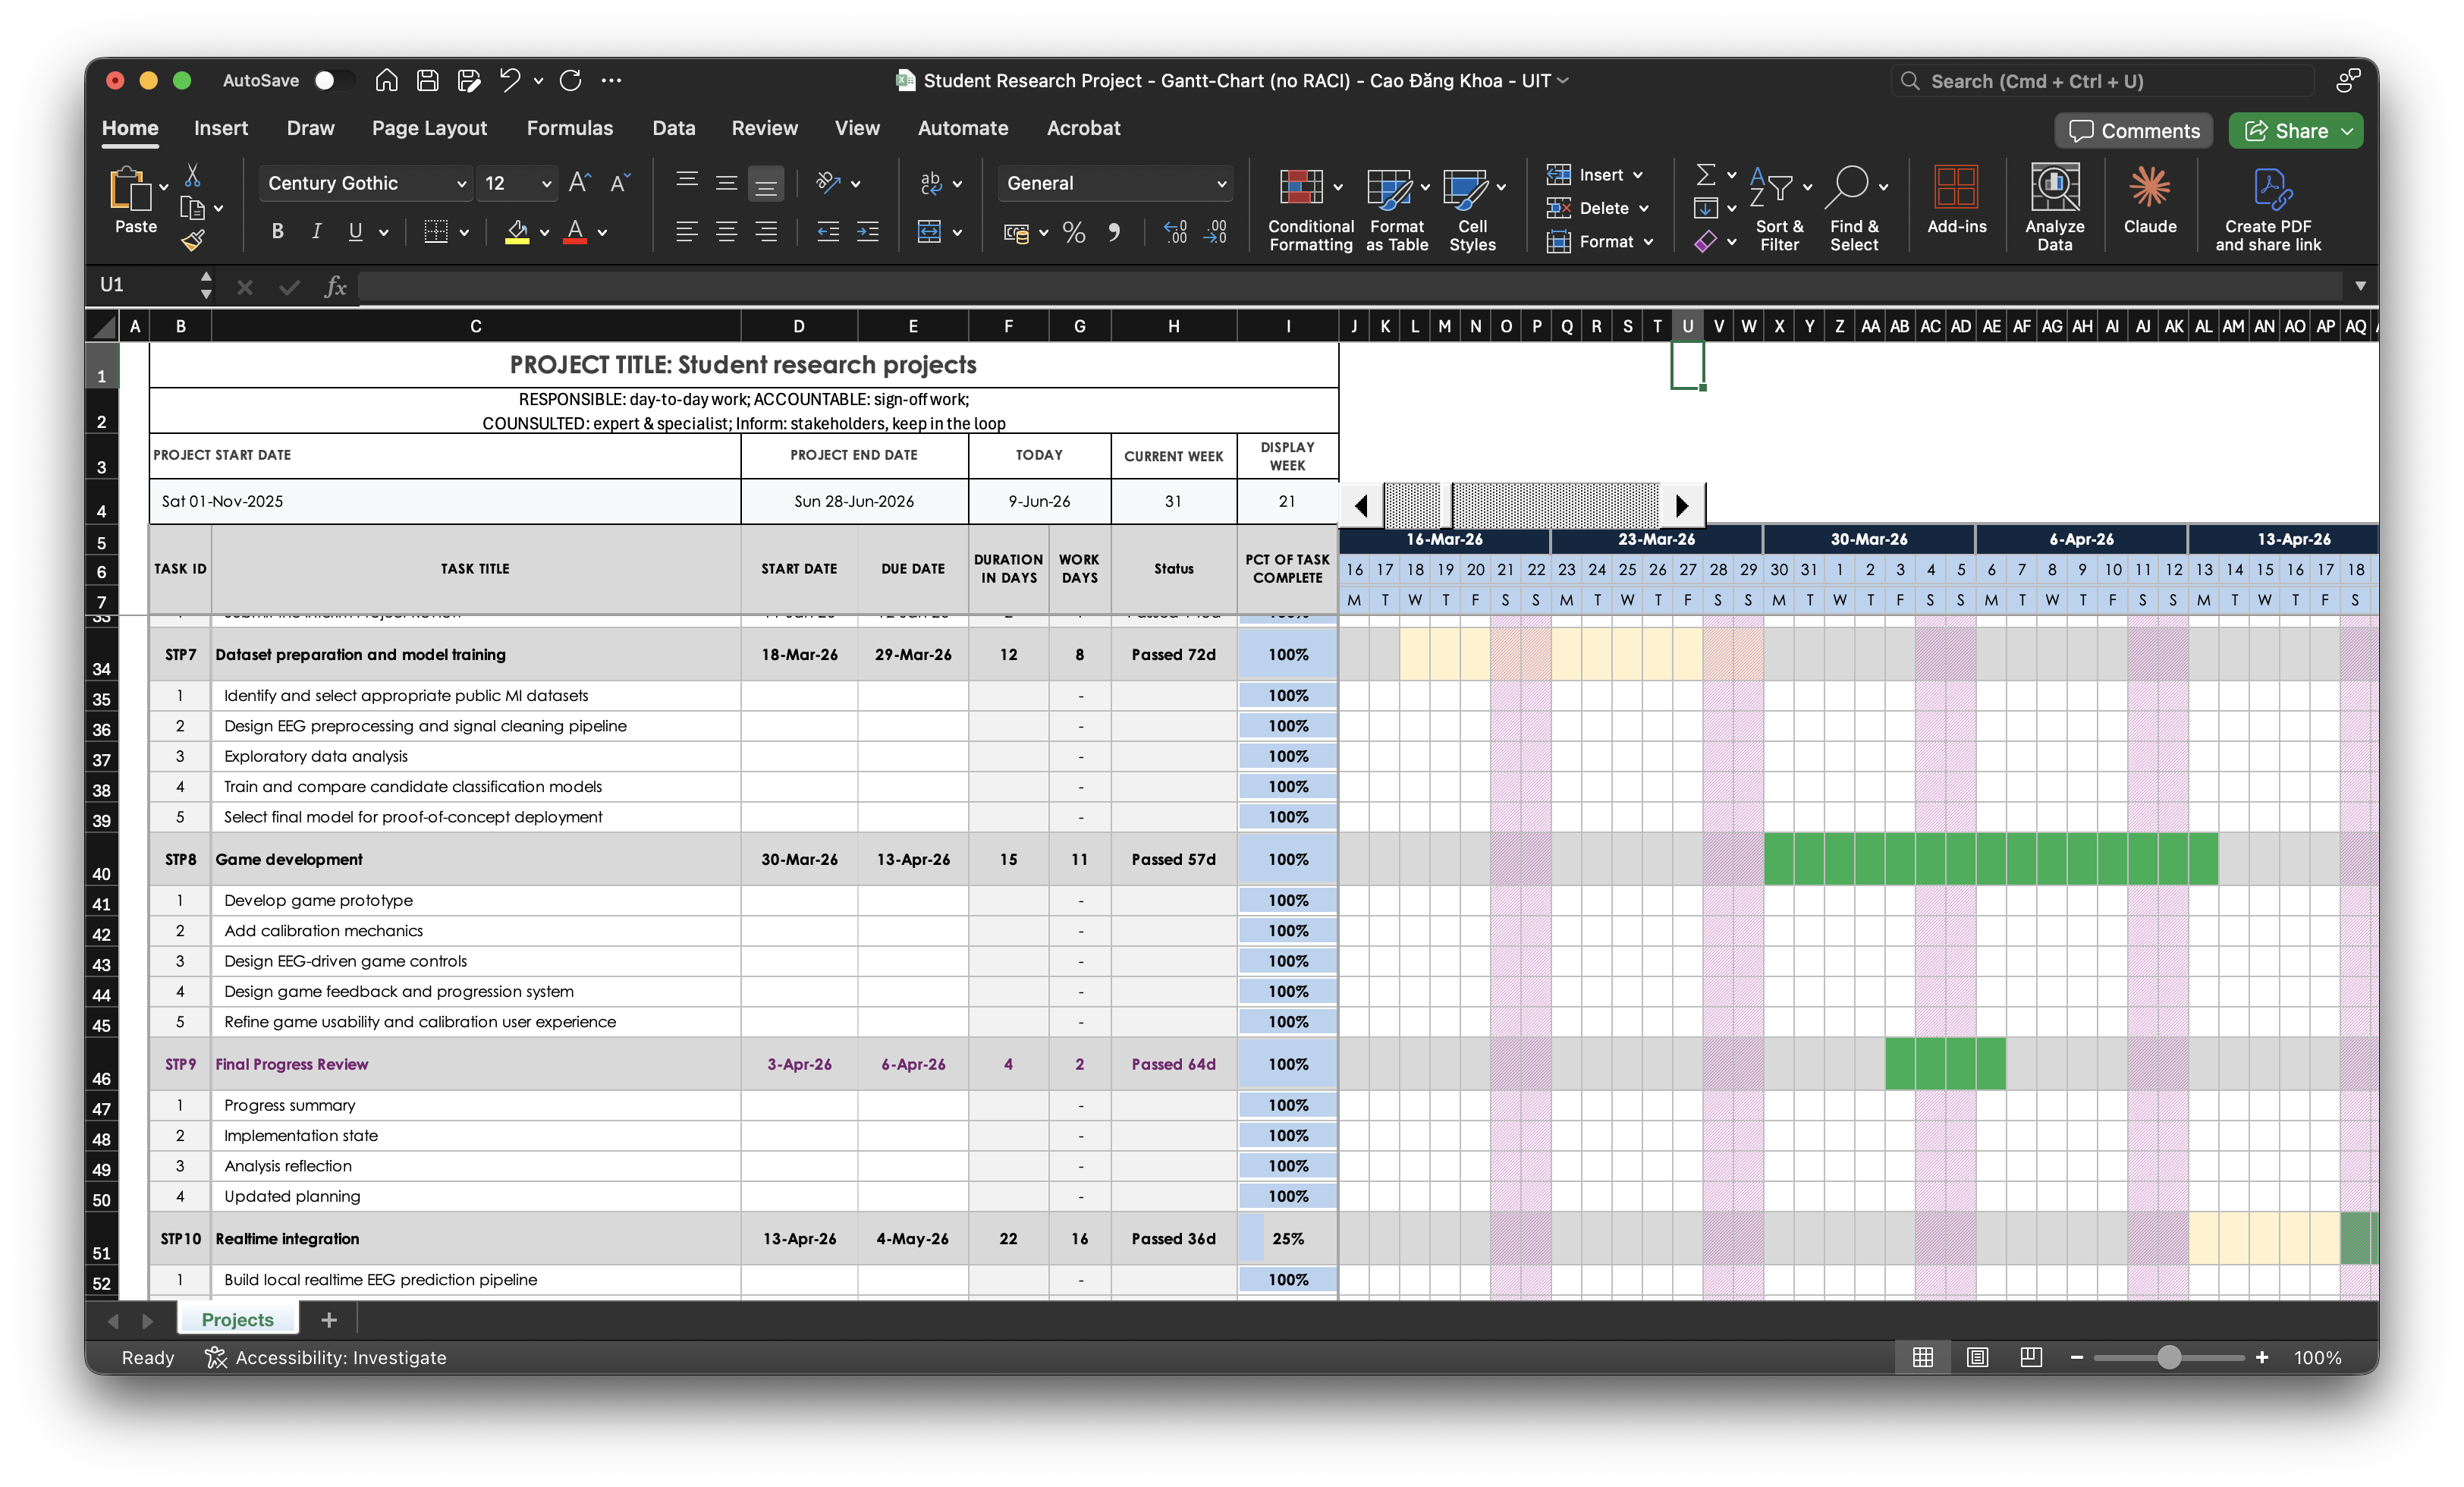
\includegraphics[width=1\textwidth]{Images/gantt-chart-new-3.png}
        \caption{Project Timeline - Part 3}
        \label{fig:gantt-chart-part-3}
    \end{figure}

    \begin{figure}[H]
        \centering
        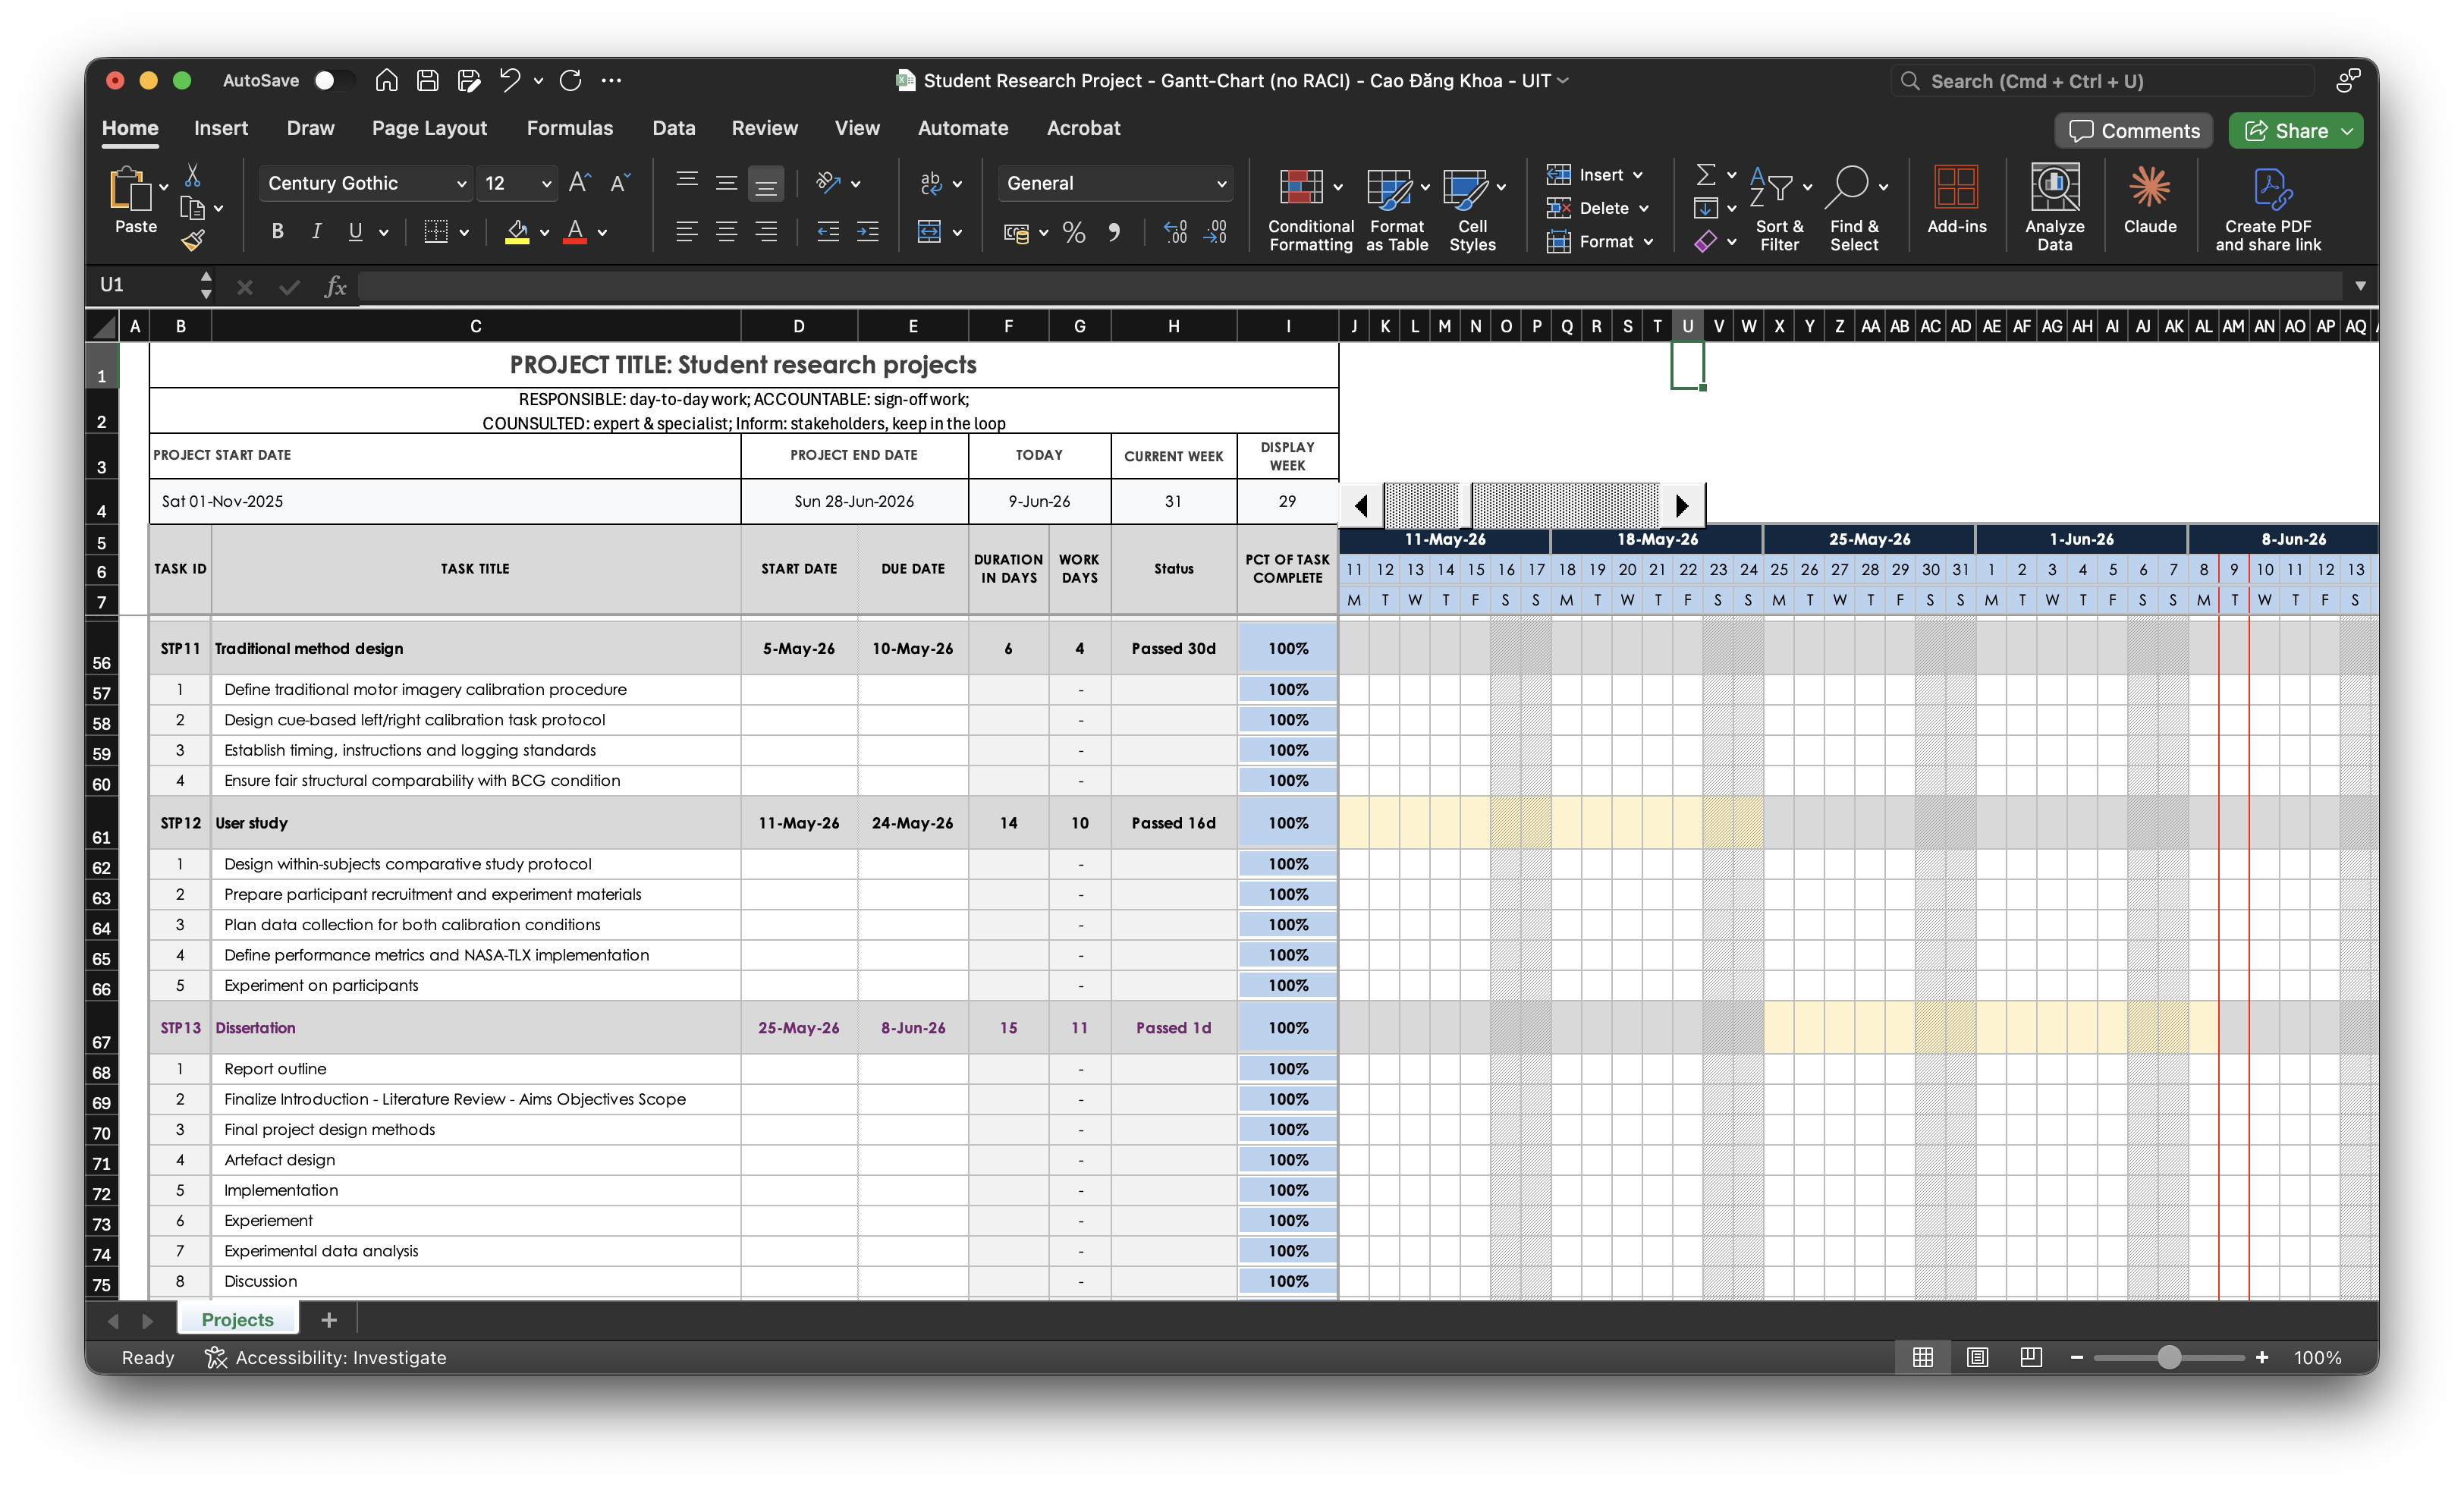
\includegraphics[width=1\textwidth]{Images/gantt-chart-new-4.png}
        \caption{Project Timeline - Part 4}
        \label{fig:gantt-chart-part-4}
    \end{figure}

    \begin{figure}[H]
        \centering
        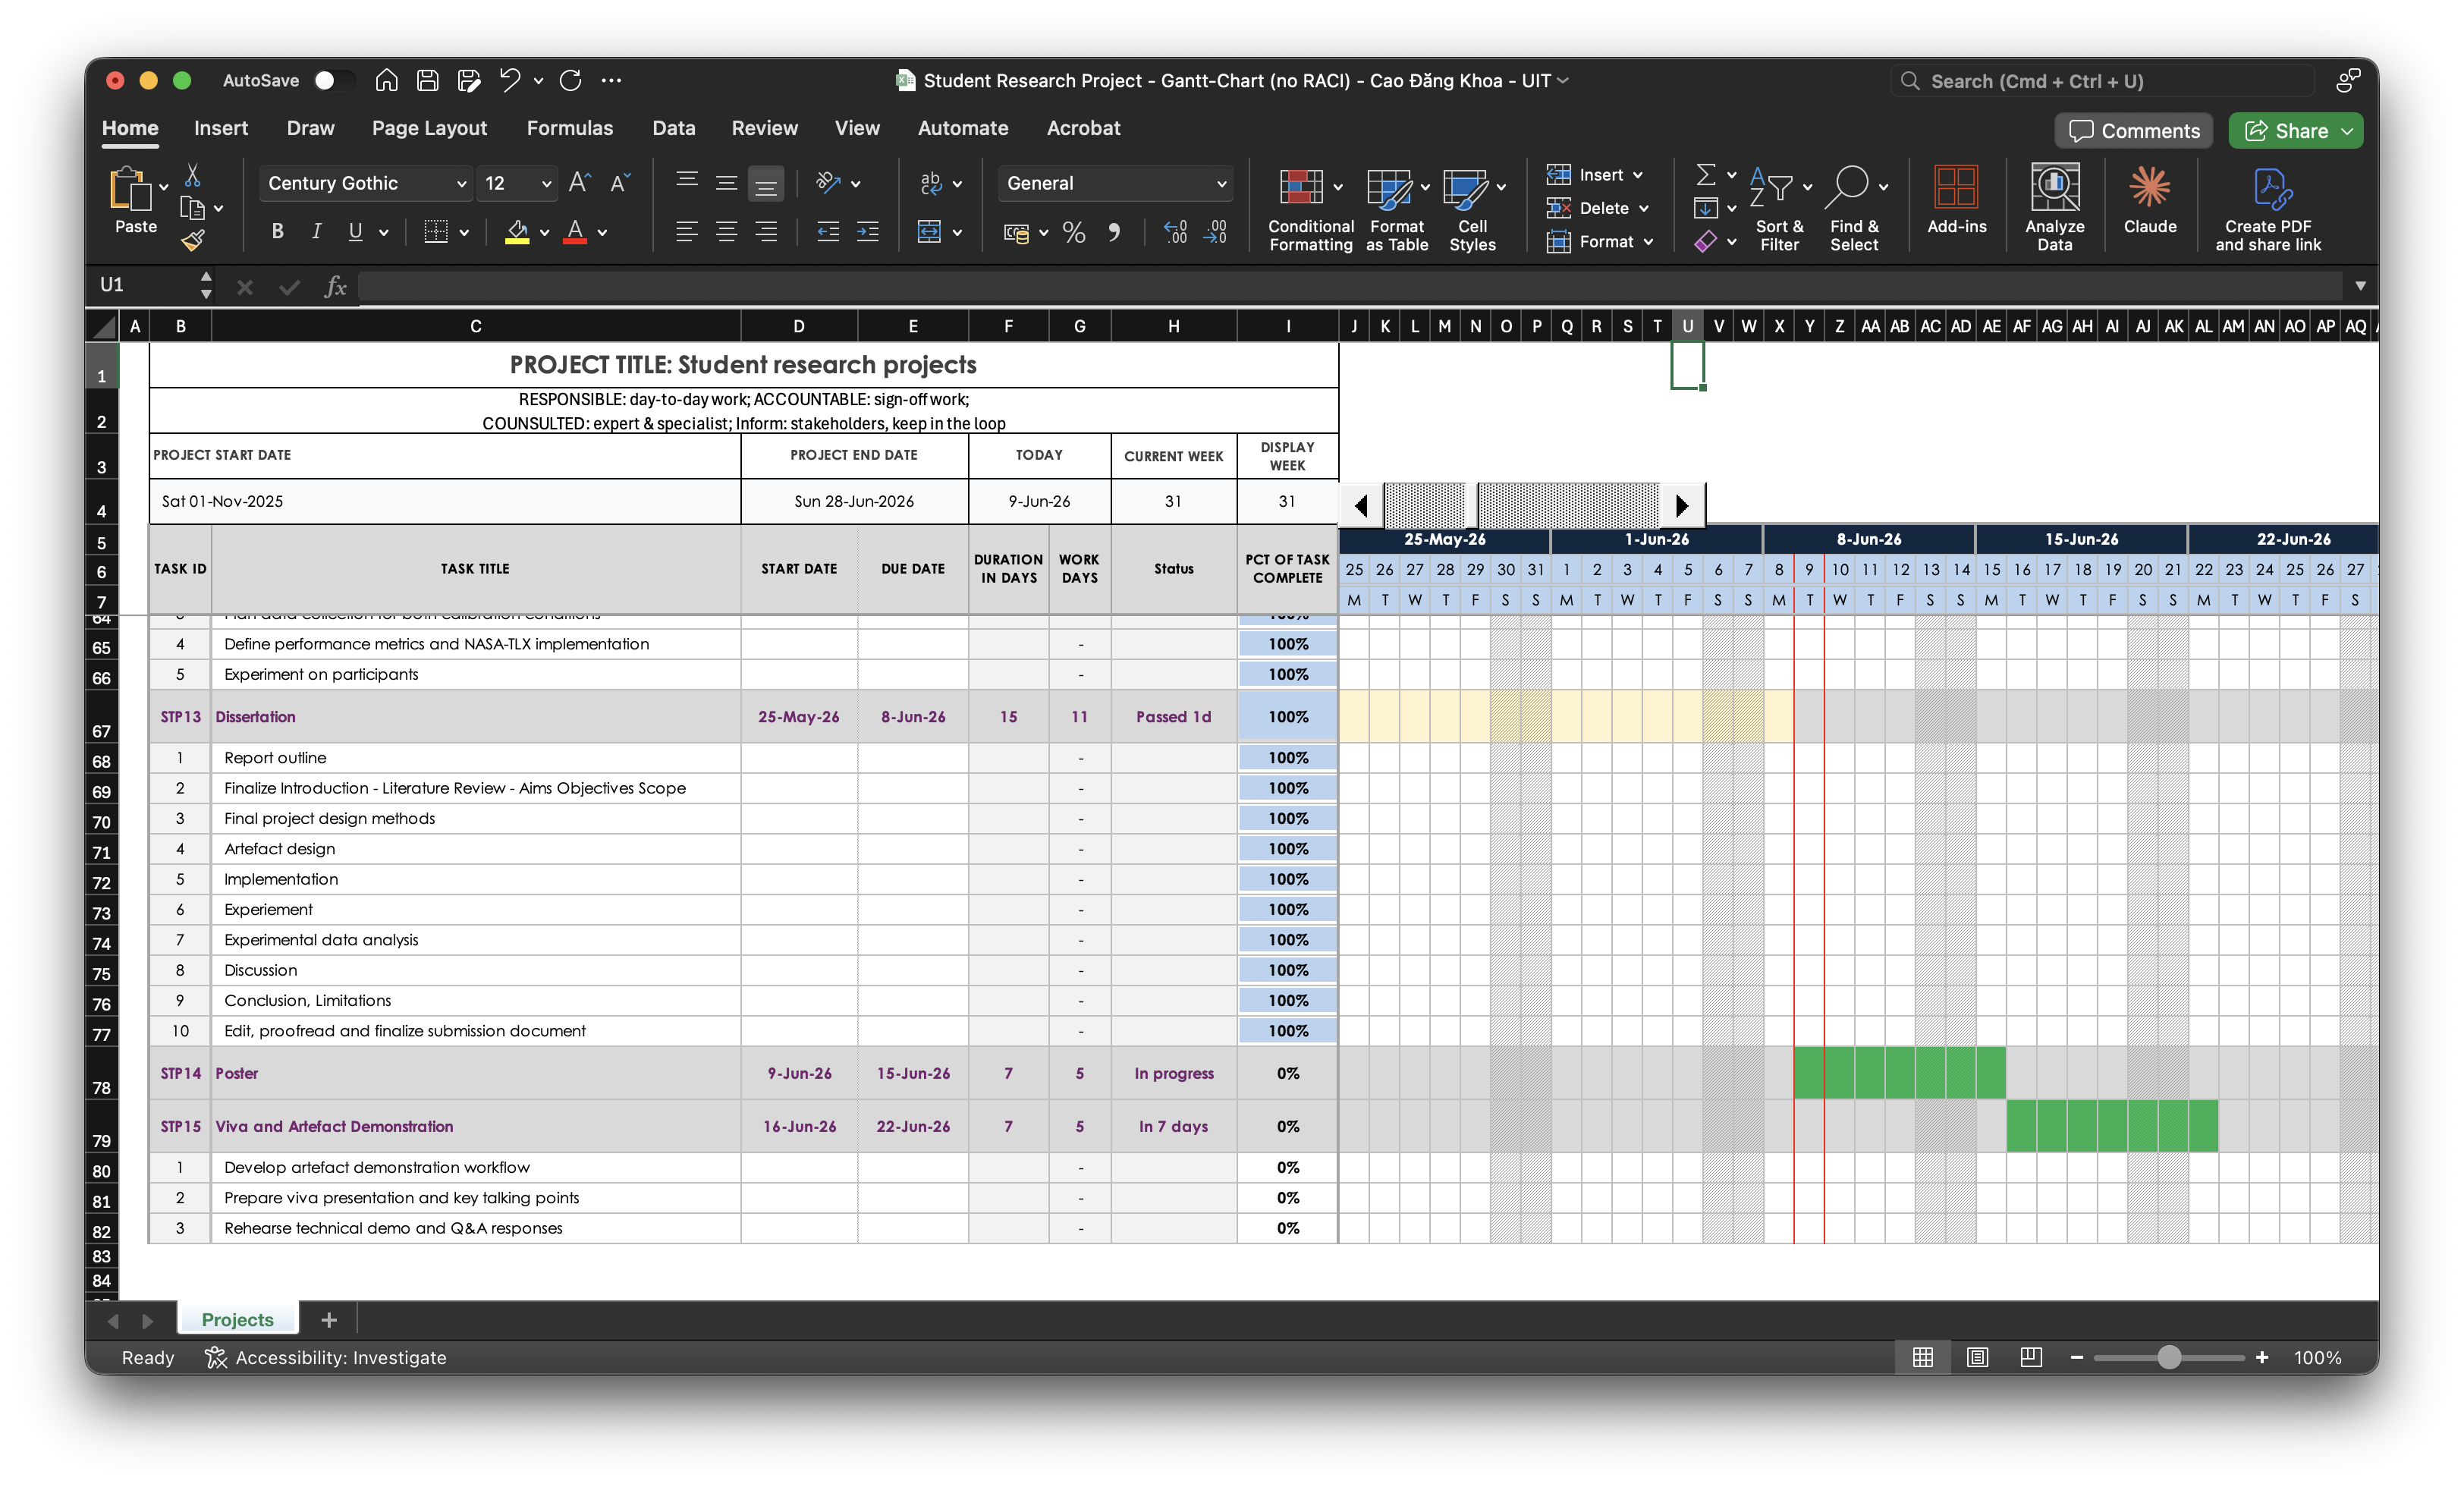
\includegraphics[width=1\textwidth]{Images/gantt-chart-new-5.png}
        \caption{Project Timeline - Part 5}
        \label{fig:gantt-chart-part-5}
    \end{figure}
    
    \section{Appendix B: Source Code Repository}

    The complete source code, artefact implementation, machine learning models, and project documentation are publicly available on GitHub: \url{https://github.com/dkhoa2906/honours-project}

    \vspace{0.5cm}
    \noindent
    The repository contains the following main components:

    \begin{itemize}
        \item \texttt{artefact/} --- Complete BCI software framework including Graz protocol interface, gamified calibration system, and live MI monitor
        
        \item \texttt{model/} --- Machine learning notebooks
        
        \item \texttt{design/} --- Logo and design materials
        
        \item \texttt{documents/} --- Project reports, weekly reports, and other project-related documents
    \end{itemize}




%------------ REFERENCES ------------%

\newpage
\vspace*{-1cm}
\chapter*{References}
\renewcommand{\bibname}{\vspace{-1cm}}
\bibliographystyle{apalike}
\bibliography{references}

\end{document}
